\documentclass[twoside]{book}

% Packages required by doxygen
\usepackage{fixltx2e}
\usepackage{calc}
\usepackage{doxygen}
\usepackage[export]{adjustbox} % also loads graphicx
\usepackage{graphicx}
\usepackage[utf8]{inputenc}
\usepackage{makeidx}
\usepackage{multicol}
\usepackage{multirow}
\PassOptionsToPackage{warn}{textcomp}
\usepackage{textcomp}
\usepackage[nointegrals]{wasysym}
\usepackage[table]{xcolor}

% Font selection
\usepackage[T1]{fontenc}
\usepackage[scaled=.90]{helvet}
\usepackage{courier}
\usepackage{amssymb}
\usepackage{sectsty}
\renewcommand{\familydefault}{\sfdefault}
\allsectionsfont{%
  \fontseries{bc}\selectfont%
  \color{darkgray}%
}
\renewcommand{\DoxyLabelFont}{%
  \fontseries{bc}\selectfont%
  \color{darkgray}%
}
\newcommand{\+}{\discretionary{\mbox{\scriptsize$\hookleftarrow$}}{}{}}

% Page & text layout
\usepackage{geometry}
\geometry{%
  a4paper,%
  top=2.5cm,%
  bottom=2.5cm,%
  left=2.5cm,%
  right=2.5cm%
}
\tolerance=750
\hfuzz=15pt
\hbadness=750
\setlength{\emergencystretch}{15pt}
\setlength{\parindent}{0cm}
\setlength{\parskip}{3ex plus 2ex minus 2ex}
\makeatletter
\renewcommand{\paragraph}{%
  \@startsection{paragraph}{4}{0ex}{-1.0ex}{1.0ex}{%
    \normalfont\normalsize\bfseries\SS@parafont%
  }%
}
\renewcommand{\subparagraph}{%
  \@startsection{subparagraph}{5}{0ex}{-1.0ex}{1.0ex}{%
    \normalfont\normalsize\bfseries\SS@subparafont%
  }%
}
\makeatother

% Headers & footers
\usepackage{fancyhdr}
\pagestyle{fancyplain}
\fancyhead[LE]{\fancyplain{}{\bfseries\thepage}}
\fancyhead[CE]{\fancyplain{}{}}
\fancyhead[RE]{\fancyplain{}{\bfseries\leftmark}}
\fancyhead[LO]{\fancyplain{}{\bfseries\rightmark}}
\fancyhead[CO]{\fancyplain{}{}}
\fancyhead[RO]{\fancyplain{}{\bfseries\thepage}}
\fancyfoot[LE]{\fancyplain{}{}}
\fancyfoot[CE]{\fancyplain{}{}}
\fancyfoot[RE]{\fancyplain{}{\bfseries\scriptsize Generated by Doxygen }}
\fancyfoot[LO]{\fancyplain{}{\bfseries\scriptsize Generated by Doxygen }}
\fancyfoot[CO]{\fancyplain{}{}}
\fancyfoot[RO]{\fancyplain{}{}}
\renewcommand{\footrulewidth}{0.4pt}
\renewcommand{\chaptermark}[1]{%
  \markboth{#1}{}%
}
\renewcommand{\sectionmark}[1]{%
  \markright{\thesection\ #1}%
}

% Indices & bibliography
\usepackage{natbib}
\usepackage[titles]{tocloft}
\setcounter{tocdepth}{3}
\setcounter{secnumdepth}{5}
\makeindex

% Hyperlinks (required, but should be loaded last)
\usepackage{ifpdf}
\ifpdf
  \usepackage[pdftex,pagebackref=true]{hyperref}
\else
  \usepackage[ps2pdf,pagebackref=true]{hyperref}
\fi
\hypersetup{%
  colorlinks=true,%
  linkcolor=blue,%
  citecolor=blue,%
  unicode%
}

% Custom commands
\newcommand{\clearemptydoublepage}{%
  \newpage{\pagestyle{empty}\cleardoublepage}%
}

\usepackage{caption}
\captionsetup{labelsep=space,justification=centering,font={bf},singlelinecheck=off,skip=4pt,position=top}

%===== C O N T E N T S =====

\begin{document}

% Titlepage & ToC
\hypersetup{pageanchor=false,
             bookmarksnumbered=true,
             pdfencoding=unicode
            }
\pagenumbering{alph}
\begin{titlepage}
\vspace*{7cm}
\begin{center}%
{\Large CoF\+:\+:Basic\+Logger }\\
\vspace*{1cm}
{\large Generated by Doxygen 1.8.13}\\
\end{center}
\end{titlepage}
\clearemptydoublepage
\pagenumbering{roman}
\tableofcontents
\clearemptydoublepage
\pagenumbering{arabic}
\hypersetup{pageanchor=true}

%--- Begin generated contents ---
\chapter{Basic Logger Module}
\label{index}\hypertarget{index}{}This is the basic logger module. Its written after the specifications stated out here. The module supports a basic logging functionality hence it is not multithreaded. This is the first draft. This logger module states out the general Logging A\+PI for basic loggers. {\itshape Single Instance Logger}

\subsection*{Basic usage}

The Logging system knows 3 different ways of logging\+:


\begin{DoxyItemize}
\item via free functions
\item via Macros
\item via a Logger Object.
\end{DoxyItemize}

Important is that the main include file for all 3 supported types is {\ttfamily \hyperlink{_logger_8h}{Logger.\+h}}.

\subsubsection*{Free Functions}

If free functions is the desired method of logging then the header file {\ttfamily \hyperlink{_logging_function_8h}{Logging\+Function.\+h}} should be enough and the desired sink {\ttfamily \hyperlink{_std_out_8h}{Sinks/\+Std\+Out.\+h}} or {\ttfamily \hyperlink{_file_8h}{Sinks/\+File.\+h}}.

{\bfseries General use}


\begin{DoxyCode}
\textcolor{preprocessor}{#include "\hyperlink{_logger_8h}{Logger.h}"}
\textcolor{keywordtype}{int} main()
\{
    cof::basic\_logger::Init<cof::basic\_logger::StdOut>(std::move(
      \hyperlink{structcof_1_1basic__logger_1_1_sink_settings}{cof::basic\_logger::SinkSettings}\{\}));
    \hyperlink{_logging_function_8h_a1f56bcf4dd7901f39b3386261c75d4a5}{cof::Log}(\textcolor{stringliteral}{"Free function Log Message"});
    \hyperlink{_logging_function_8h_ac0c0af18a99bcd635fb89679890cdeaa}{cof::Warn}(\textcolor{stringliteral}{"Free function Warn Message"});
    \hyperlink{_logging_function_8h_a4d2fa4bc5cade7fdb692a0615b489997}{cof::Info}(\textcolor{stringliteral}{"Free function Info Message"});
    \hyperlink{_logging_function_8h_ac0fff05470889b9bf801966564dddb36}{cof::Debug}(\textcolor{stringliteral}{"Free function Debug Message"});
    \hyperlink{_logging_function_8h_a09fbfa2e340f6dff1804c2a19a7b34f4}{cof::Error}(\textcolor{stringliteral}{"Free function Error Message"});
    cof::basic\_logger::Deint();

    \textcolor{keywordflow}{return} 0;
\}
\end{DoxyCode}


{\bfseries With helper functions\+:}


\begin{DoxyCode}
\textcolor{preprocessor}{#include "\hyperlink{_logger_8h}{Logger.h}"}
\textcolor{keywordtype}{int} main()
\{
    cof::basic\_logger::InitStdOut();
    \hyperlink{_logging_function_8h_a1f56bcf4dd7901f39b3386261c75d4a5}{cof::Log}(\textcolor{stringliteral}{"Free function Log Message"});
    \hyperlink{_logging_function_8h_ac0c0af18a99bcd635fb89679890cdeaa}{cof::Warn}(\textcolor{stringliteral}{"Free function Warn Message"});
    \hyperlink{_logging_function_8h_a4d2fa4bc5cade7fdb692a0615b489997}{cof::Info}(\textcolor{stringliteral}{"Free function Info Message"});
    \hyperlink{_logging_function_8h_ac0fff05470889b9bf801966564dddb36}{cof::Debug}(\textcolor{stringliteral}{"Free function Debug Message"});
    \hyperlink{_logging_function_8h_a09fbfa2e340f6dff1804c2a19a7b34f4}{cof::Error}(\textcolor{stringliteral}{"Free function Error Message"});
    cof::basic\_logger::Deint();

    \textcolor{keywordflow}{return} 0;
\}
\end{DoxyCode}



\begin{DoxyCode}
\textcolor{preprocessor}{#include "\hyperlink{_logger_8h}{Logger.h}"}
\textcolor{keywordtype}{int} main()
\{
    cof::basic\_logger::InitFile(\hyperlink{structcof_1_1basic__logger_1_1_file_sink_settings}{cof::basic\_logger::FileSinkSettings}\{ \textcolor{stringliteral}{"
      log.txt"} \});
    \hyperlink{_logging_function_8h_a1f56bcf4dd7901f39b3386261c75d4a5}{cof::Log}(\textcolor{stringliteral}{"Free function Log Message"});
    \hyperlink{_logging_function_8h_ac0c0af18a99bcd635fb89679890cdeaa}{cof::Warn}(\textcolor{stringliteral}{"Free function Warn Message"});
    \hyperlink{_logging_function_8h_a4d2fa4bc5cade7fdb692a0615b489997}{cof::Info}(\textcolor{stringliteral}{"Free function Info Message"});
    \hyperlink{_logging_function_8h_ac0fff05470889b9bf801966564dddb36}{cof::Debug}(\textcolor{stringliteral}{"Free function Debug Message"});
    \hyperlink{_logging_function_8h_a09fbfa2e340f6dff1804c2a19a7b34f4}{cof::Error}(\textcolor{stringliteral}{"Free function Error Message"});
    cof::basic\_logger::Deint();

    \textcolor{keywordflow}{return} 0;
\}
\end{DoxyCode}


\subsubsection*{Macros}

If free functions is the desired method of logging then the header file {\ttfamily Logging\+Macro.\+h} should be enough and the desired sink {\ttfamily \hyperlink{_std_out_8h}{Sinks/\+Std\+Out.\+h}} or {\ttfamily \hyperlink{_file_8h}{Sinks/\+File.\+h}}.


\begin{DoxyCode}
\textcolor{preprocessor}{#include "\hyperlink{_logger_8h}{Logger.h}"}

\textcolor{keywordtype}{int} main()
\{
    LOGGER\_INIT\_STDOUT()
    \hyperlink{_logging_macros_8h_a018a1fe4b078f1a684610657a5848860}{LOG}("Macro Log Message")
    \hyperlink{_logging_macros_8h_a5dd0aa9e28b0c7db286181cfc81ebb94}{WARN}("Macro Warn Message")
    \hyperlink{_logging_macros_8h_aafc148cee6d6c9e76b4ef417c7056f8f}{INFO}("Macro Info Message")
    \hyperlink{_logging_macros_8h_a614c336056da6e8a7e6a06ed991b9feb}{DEBUG}("Macro Debug Message")
    \hyperlink{_logging_macros_8h_a78e40dfd87f516e322340d249027aea1}{ERROR}("Macro Error Message")
    \hyperlink{_logging_macros_8h_a949408ae41659956042cdbe1e59281f3}{LOGGER\_DEINIT}

    return 0;
\}
\end{DoxyCode}


\subsubsection*{Object}

If free functions is the desired method of logging then the header file {\ttfamily \hyperlink{_basic_logger_8h}{Basic\+Logger.\+h}} should be enough and the desired sink {\ttfamily \hyperlink{_std_out_8h}{Sinks/\+Std\+Out.\+h}} or {\ttfamily \hyperlink{_file_8h}{Sinks/\+File.\+h}}.


\begin{DoxyCode}
\textcolor{preprocessor}{#include "\hyperlink{_logger_8h}{Logger.h}"}

\textcolor{keyword}{class }OtherClass
\{
\textcolor{keyword}{public}:
    \textcolor{keyword}{explicit} OtherClass(\hyperlink{classcof_1_1basic__logger_1_1_logger}{cof::basic\_logger::Logger}& logger);

    \textcolor{keywordtype}{void} some\_action();
\textcolor{keyword}{private}:
    \hyperlink{classcof_1_1basic__logger_1_1_logger}{cof::basic\_logger::Logger}& logger\_;
\};

OtherClass::OtherClass(\hyperlink{classcof_1_1basic__logger_1_1_logger}{cof::basic\_logger::Logger}& logger) : logger\_(logger)
\{
\}

\textcolor{keywordtype}{void} OtherClass::some\_action()
\{
    logger\_.Debug(\textcolor{stringliteral}{"I am doing something"});
\}

\textcolor{keyword}{class }Application
\{
\textcolor{keyword}{public}:
    Application(\hyperlink{classcof_1_1basic__logger_1_1_logger}{cof::basic\_logger::Logger}&& logger);
    \textcolor{keywordtype}{void} do\_something();
\textcolor{keyword}{private}:
    \hyperlink{classcof_1_1basic__logger_1_1_logger}{cof::basic\_logger::Logger} logger\_;
    OtherClass action\_;
\};

Application::Application(\hyperlink{classcof_1_1basic__logger_1_1_logger}{cof::basic\_logger::Logger}&& logger): logger\_(std::move(
      logger)), action\_(logger\_)
\{
\}

\textcolor{keywordtype}{void} Application::do\_something()
\{
    logger\_.Info(\textcolor{stringliteral}{"I am doing something"});
    action\_.some\_action();
\}



\textcolor{keywordtype}{int} main()
\{
    \textcolor{keyword}{auto}* sink = \textcolor{keyword}{new} \hyperlink{classcof_1_1basic__logger_1_1_std_out}{cof::basic\_logger::StdOut}(\textcolor{keyword}{new} 
      \hyperlink{structcof_1_1basic__logger_1_1_sink_settings}{cof::basic\_logger::SinkSettings});
    \textcolor{comment}{// takes the ownership of the pointer.}
    \textcolor{keyword}{auto} logger = \hyperlink{classcof_1_1basic__logger_1_1_logger}{cof::basic\_logger::Logger}(sink);

    Application app(std::move(logger));
    app.do\_something();

    \textcolor{keywordflow}{return} 0;
\}
\end{DoxyCode}


\subsection*{Why the nested namespace {\ttfamily basic\+\_\+logger}}

The reason for this is to clearly state out that this is the {\ttfamily basic\+\_\+logger} and that this module cannot be interchanged with another logger.

Example for demonstrating the problem\+:


\begin{DoxyCode}
\textcolor{comment}{//complex logger API}
cof::logger::InitStdOut(\textcolor{stringliteral}{"name"});
\hyperlink{_logging_function_8h_a1f56bcf4dd7901f39b3386261c75d4a5}{cof::Log}(\textcolor{stringliteral}{"Name"},\textcolor{stringliteral}{"Log message"});
\end{DoxyCode}


Simple Logger\+:


\begin{DoxyCode}
cof::basic\_logger::InitStdOut();    
\hyperlink{_logging_function_8h_a1f56bcf4dd7901f39b3386261c75d4a5}{cof::Log}(\textcolor{stringliteral}{"Free function Log Message"});
\end{DoxyCode}
 
\chapter{Technical Specification}
\label{md__a_1_collectionofframeworks__basic_logger_ts}
\Hypertarget{md__a_1_collectionofframeworks__basic_logger_ts}
This document shall describe the technical specification of the Basic Logger module.

\subsection*{Design Goal}

The design goal of this module is it to deliver a simple none multithreaded logger interface which is easy to use and supports formatting.

\subsection*{The Interface}

The logger A\+PI shall cover 3 different approaches\+:


\begin{DoxyItemize}
\item free functions
\item a {\ttfamily Logger} class
\item Logger Macros
\end{DoxyItemize}

Each of those approaches shall have the same set of functions.


\begin{DoxyItemize}
\item {\ttfamily Log(format,\mbox{[}information\mbox{]})}
\item {\ttfamily Info(format,\mbox{[}information\mbox{]})}
\item {\ttfamily Debug(format,\mbox{[}information\mbox{]})}
\item {\ttfamily Warn(format,\mbox{[}information\mbox{]})}
\item {\ttfamily Error(format,\mbox{[}information\mbox{]})}
\end{DoxyItemize}

{\bfseries Activation specification}

The Module only works if one of the following pre-\/processor defines is defined\+:

{\ttfamily D\+E\+B\+UG , D\+E\+B\+U\+G\+\_\+ , \+\_\+\+D\+E\+B\+U\+G\+\_\+ , D\+E\+B\+U\+G\+\_\+ , \+\_\+\+D\+E\+B\+UG, C\+O\+F\+\_\+\+U\+S\+E\+\_\+\+L\+O\+G\+G\+ER}

if they are not defined the Logging class will be empty. {\ttfamily size 1} and the free function will be empty as well. No zero overhead.

{\bfseries Macro specification}

They shall be capitalized and always print the {\ttfamily \+\_\+\+\_\+\+F\+I\+L\+E\+\_\+\+\_\+} and {\ttfamily \+\_\+\+\_\+\+L\+I\+N\+E\+\_\+\+\_\+} with its output unless {\ttfamily C\+O\+F\+\_\+\+L\+O\+G\+G\+E\+R\+\_\+\+U\+S\+E\+\_\+\+D\+A\+T\+E\+\_\+\+L\+I\+NE} is not defined. If {\ttfamily C\+O\+F\+\_\+\+L\+O\+G\+G\+E\+R\+\_\+\+U\+S\+E\+\_\+\+D\+A\+T\+E\+\_\+\+L\+I\+NE} is undefined there shall be no output of the current line and file.

{\bfseries Output specification}

The output on the screen shall be as following\+:


\begin{DoxyCode}
[Level] [Date Time] [[File] [Line]] [Message]
\end{DoxyCode}


example\+:


\begin{DoxyCode}
[Info] [21-02-2018 22:03] </home/user/cpp/test.cpp:24> User data was empty used default.
\end{DoxyCode}


{\bfseries Sink Specification}

A {\ttfamily Sink} is a class which provides the low level function such as {\ttfamily print} on screen or save the output in a file. In this basic approach the {\ttfamily Sink} {\itshape cannot} be changes during runtime after its set.

The basic sinks the system shall support are\+:


\begin{DoxyItemize}
\item Standard in / out (Terminal)
\item File
\item Both 
\end{DoxyItemize}
\chapter{Module Index}
\section{Modules}
Here is a list of all modules\+:\begin{DoxyCompactList}
\item \contentsline{section}{Sinks}{\pageref{group___sinks}}{}
\item \contentsline{section}{Sink Settings}{\pageref{group___sinks___settings}}{}
\end{DoxyCompactList}

\chapter{Hierarchical Index}
\section{Class Hierarchy}
This inheritance list is sorted roughly, but not completely, alphabetically\+:\begin{DoxyCompactList}
\item \contentsline{section}{cof\+:\+:basic\+\_\+logger\+:\+:Logger}{\pageref{classcof_1_1basic__logger_1_1_logger}}{}
\item \contentsline{section}{cof\+:\+:basic\+\_\+logger\+:\+:Sink}{\pageref{classcof_1_1basic__logger_1_1_sink}}{}
\begin{DoxyCompactList}
\item \contentsline{section}{cof\+:\+:basic\+\_\+logger\+:\+:File}{\pageref{classcof_1_1basic__logger_1_1_file}}{}
\item \contentsline{section}{cof\+:\+:basic\+\_\+logger\+:\+:Std\+Out}{\pageref{classcof_1_1basic__logger_1_1_std_out}}{}
\end{DoxyCompactList}
\item \contentsline{section}{cof\+:\+:basic\+\_\+logger\+:\+:Sink\+Settings}{\pageref{structcof_1_1basic__logger_1_1_sink_settings}}{}
\begin{DoxyCompactList}
\item \contentsline{section}{cof\+:\+:basic\+\_\+logger\+:\+:File\+Sink\+Settings}{\pageref{structcof_1_1basic__logger_1_1_file_sink_settings}}{}
\end{DoxyCompactList}
\end{DoxyCompactList}

\chapter{Class Index}
\section{Class List}
Here are the classes, structs, unions and interfaces with brief descriptions\+:\begin{DoxyCompactList}
\item\contentsline{section}{\hyperlink{classcof_1_1basic__logger_1_1_file}{cof\+::basic\+\_\+logger\+::\+File} \\*The actual \hyperlink{classcof_1_1basic__logger_1_1_file}{File} logger }{\pageref{classcof_1_1basic__logger_1_1_file}}{}
\item\contentsline{section}{\hyperlink{structcof_1_1basic__logger_1_1_file_sink_settings}{cof\+::basic\+\_\+logger\+::\+File\+Sink\+Settings} \\*Defines settings for the \hyperlink{classcof_1_1basic__logger_1_1_file}{File} logger }{\pageref{structcof_1_1basic__logger_1_1_file_sink_settings}}{}
\item\contentsline{section}{\hyperlink{classcof_1_1basic__logger_1_1_logger}{cof\+::basic\+\_\+logger\+::\+Logger} \\*A basic non multi threaded logger }{\pageref{classcof_1_1basic__logger_1_1_logger}}{}
\item\contentsline{section}{\hyperlink{classcof_1_1basic__logger_1_1_sink}{cof\+::basic\+\_\+logger\+::\+Sink} \\*The Base \hyperlink{classcof_1_1basic__logger_1_1_sink}{Sink} class }{\pageref{classcof_1_1basic__logger_1_1_sink}}{}
\item\contentsline{section}{\hyperlink{structcof_1_1basic__logger_1_1_sink_settings}{cof\+::basic\+\_\+logger\+::\+Sink\+Settings} \\*The Base \hyperlink{structcof_1_1basic__logger_1_1_sink_settings}{Sink\+Settings} class }{\pageref{structcof_1_1basic__logger_1_1_sink_settings}}{}
\item\contentsline{section}{\hyperlink{classcof_1_1basic__logger_1_1_std_out}{cof\+::basic\+\_\+logger\+::\+Std\+Out} \\*Terminal logging }{\pageref{classcof_1_1basic__logger_1_1_std_out}}{}
\end{DoxyCompactList}

\chapter{File Index}
\section{File List}
Here is a list of all documented files with brief descriptions\+:\begin{DoxyCompactList}
\item\contentsline{section}{A\+:/collectionofframeworks/\+Basic\+Logger/include/\hyperlink{_basic_logger_8h}{Basic\+Logger.\+h} \\*Contains the basic impl of the logger class }{\pageref{_basic_logger_8h}}{}
\item\contentsline{section}{A\+:/collectionofframeworks/\+Basic\+Logger/include/\hyperlink{_logger_8h}{Logger.\+h} \\*Easy to include file }{\pageref{_logger_8h}}{}
\item\contentsline{section}{A\+:/collectionofframeworks/\+Basic\+Logger/include/\hyperlink{_logging_function_8h}{Logging\+Function.\+h} \\*A collection of logging free functions }{\pageref{_logging_function_8h}}{}
\item\contentsline{section}{A\+:/collectionofframeworks/\+Basic\+Logger/include/\hyperlink{_logging_macros_8h}{Logging\+Macros.\+h} \\*A collection of logging Macros which resolve into free functions }{\pageref{_logging_macros_8h}}{}
\item\contentsline{section}{A\+:/collectionofframeworks/\+Basic\+Logger/include/\+Sinks/\hyperlink{_file_8h}{File.\+h} \\*File Sink and File\+Sink Settings are defined here }{\pageref{_file_8h}}{}
\item\contentsline{section}{A\+:/collectionofframeworks/\+Basic\+Logger/include/\+Sinks/\hyperlink{_sink_8h}{Sink.\+h} \\*Sink class as well as {\ttfamily Level enum class} }{\pageref{_sink_8h}}{}
\item\contentsline{section}{A\+:/collectionofframeworks/\+Basic\+Logger/include/\+Sinks/\hyperlink{_std_out_8h}{Std\+Out.\+h} \\*Terminal Sink }{\pageref{_std_out_8h}}{}
\end{DoxyCompactList}

\chapter{Module Documentation}
\hypertarget{group___sinks}{}\section{Sinks}
\label{group___sinks}\index{Sinks@{Sinks}}


Logger backend.  


\subsection*{Classes}
\begin{DoxyCompactItemize}
\item 
class \hyperlink{classcof_1_1basic__logger_1_1_file}{cof\+::basic\+\_\+logger\+::\+File}
\begin{DoxyCompactList}\small\item\em The actual \hyperlink{classcof_1_1basic__logger_1_1_file}{File} logger. \end{DoxyCompactList}\item 
class \hyperlink{classcof_1_1basic__logger_1_1_sink}{cof\+::basic\+\_\+logger\+::\+Sink}
\begin{DoxyCompactList}\small\item\em The Base \hyperlink{classcof_1_1basic__logger_1_1_sink}{Sink} class. \end{DoxyCompactList}\item 
class \hyperlink{classcof_1_1basic__logger_1_1_std_out}{cof\+::basic\+\_\+logger\+::\+Std\+Out}
\begin{DoxyCompactList}\small\item\em Terminal logging. \end{DoxyCompactList}\end{DoxyCompactItemize}


\subsection{Detailed Description}
Logger backend. 

Sinks are the objects that actually write the log to their target. Each sink should be responsible for only single target (e.\+g file, console, db). 
\hypertarget{group___sinks___settings}{}\section{Sink Settings}
\label{group___sinks___settings}\index{Sink Settings@{Sink Settings}}


Settings for Sinks.  


\subsection*{Classes}
\begin{DoxyCompactItemize}
\item 
struct \hyperlink{structcof_1_1basic__logger_1_1_file_sink_settings}{cof\+::basic\+\_\+logger\+::\+File\+Sink\+Settings}
\begin{DoxyCompactList}\small\item\em Defines settings for the \hyperlink{classcof_1_1basic__logger_1_1_file}{File} logger. \end{DoxyCompactList}\item 
struct \hyperlink{structcof_1_1basic__logger_1_1_sink_settings}{cof\+::basic\+\_\+logger\+::\+Sink\+Settings}
\begin{DoxyCompactList}\small\item\em The Base \hyperlink{structcof_1_1basic__logger_1_1_sink_settings}{Sink\+Settings} class. \end{DoxyCompactList}\end{DoxyCompactItemize}


\subsection{Detailed Description}
Settings for Sinks. 

Define how Sinks can behave. For example what file the sink should log to etc. 
\chapter{Class Documentation}
\hypertarget{classcof_1_1basic__logger_1_1_file}{}\section{cof\+:\+:basic\+\_\+logger\+:\+:File Class Reference}
\label{classcof_1_1basic__logger_1_1_file}\index{cof\+::basic\+\_\+logger\+::\+File@{cof\+::basic\+\_\+logger\+::\+File}}


The actual \hyperlink{classcof_1_1basic__logger_1_1_file}{File} logger.  




{\ttfamily \#include $<$File.\+h$>$}

Inheritance diagram for cof\+:\+:basic\+\_\+logger\+:\+:File\+:\begin{figure}[H]
\begin{center}
\leavevmode
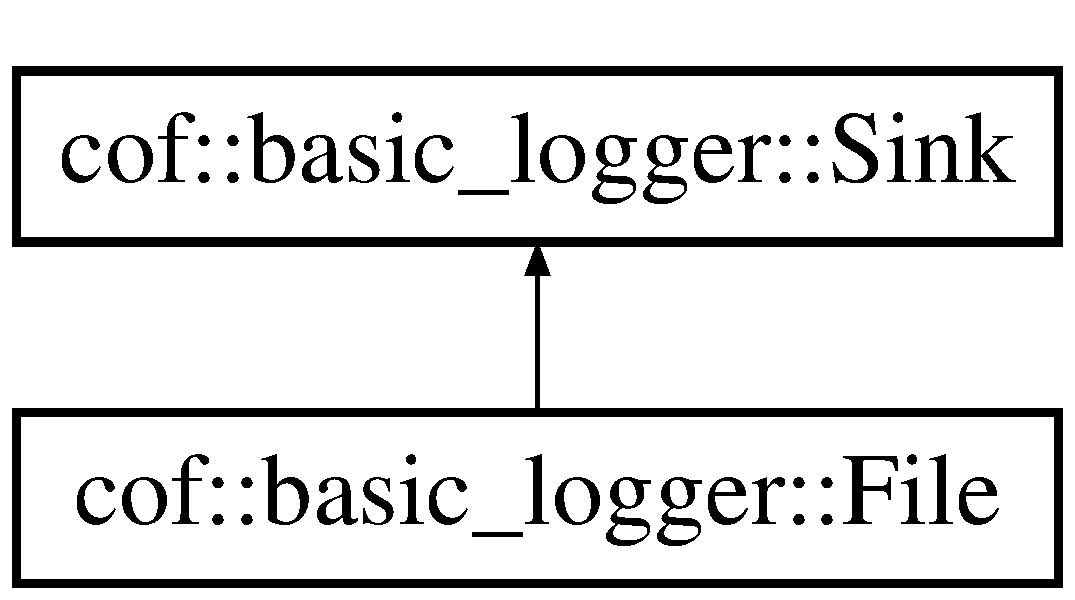
\includegraphics[height=2.000000cm]{classcof_1_1basic__logger_1_1_file}
\end{center}
\end{figure}
\subsection*{Public Member Functions}
\begin{DoxyCompactItemize}
\item 
\mbox{\Hypertarget{classcof_1_1basic__logger_1_1_file_a01bf70f50c3de009072764006194727c}\label{classcof_1_1basic__logger_1_1_file_a01bf70f50c3de009072764006194727c}} 
{\bfseries File} (\hyperlink{structcof_1_1basic__logger_1_1_sink_settings}{Sink\+Settings} $\ast$settings)
\end{DoxyCompactItemize}
\subsection*{Protected Member Functions}
\begin{DoxyCompactItemize}
\item 
\mbox{\Hypertarget{classcof_1_1basic__logger_1_1_file_a057640c6e84ddffd35215dee11e5f6a7}\label{classcof_1_1basic__logger_1_1_file_a057640c6e84ddffd35215dee11e5f6a7}} 
virtual void {\bfseries Process} (Level lvl, fmt\+::memory\+\_\+buffer \&\&buffer) override final
\end{DoxyCompactItemize}
\subsection*{Private Attributes}
\begin{DoxyCompactItemize}
\item 
\mbox{\Hypertarget{classcof_1_1basic__logger_1_1_file_a27e2decc7e6b477428c6cc3953cb31fd}\label{classcof_1_1basic__logger_1_1_file_a27e2decc7e6b477428c6cc3953cb31fd}} 
\hyperlink{structcof_1_1basic__logger_1_1_file_sink_settings}{File\+Sink\+Settings} {\bfseries settings\+\_\+}
\item 
\mbox{\Hypertarget{classcof_1_1basic__logger_1_1_file_acd3d0aa11a2a7369553eef83ee12710d}\label{classcof_1_1basic__logger_1_1_file_acd3d0aa11a2a7369553eef83ee12710d}} 
F\+I\+LE $\ast$ {\bfseries file\+\_\+}
\end{DoxyCompactItemize}
\subsection*{Additional Inherited Members}


\subsection{Detailed Description}
The actual \hyperlink{classcof_1_1basic__logger_1_1_file}{File} logger. 

Logs to a specified file with {\ttfamily fwrite} and {\ttfamily File$\ast$}. This class uses R\+A\+II. Hence {\ttfamily $\sim$\+File} is cleaning up the mess.

\begin{DoxyAuthor}{Author}
Simon Renger 
\end{DoxyAuthor}
\begin{DoxyVersion}{Version}
1.\+0 
\end{DoxyVersion}
\begin{DoxyDate}{Date}
2018 
\end{DoxyDate}
\begin{DoxyCopyright}{Copyright}
The M\+IT License 
\end{DoxyCopyright}


The documentation for this class was generated from the following files\+:\begin{DoxyCompactItemize}
\item 
A\+:/collectionofframeworks/\+Basic\+Logger/include/\+Sinks/\hyperlink{_file_8h}{File.\+h}\item 
A\+:/collectionofframeworks/\+Basic\+Logger/src/\+Sinks/File.\+cpp\end{DoxyCompactItemize}

\hypertarget{structcof_1_1basic__logger_1_1_file_sink_settings}{}\section{cof\+:\+:basic\+\_\+logger\+:\+:File\+Sink\+Settings Struct Reference}
\label{structcof_1_1basic__logger_1_1_file_sink_settings}\index{cof\+::basic\+\_\+logger\+::\+File\+Sink\+Settings@{cof\+::basic\+\_\+logger\+::\+File\+Sink\+Settings}}


Defines settings for the \hyperlink{classcof_1_1basic__logger_1_1_file}{File} logger.  




{\ttfamily \#include $<$File.\+h$>$}

Inheritance diagram for cof\+:\+:basic\+\_\+logger\+:\+:File\+Sink\+Settings\+:\begin{figure}[H]
\begin{center}
\leavevmode
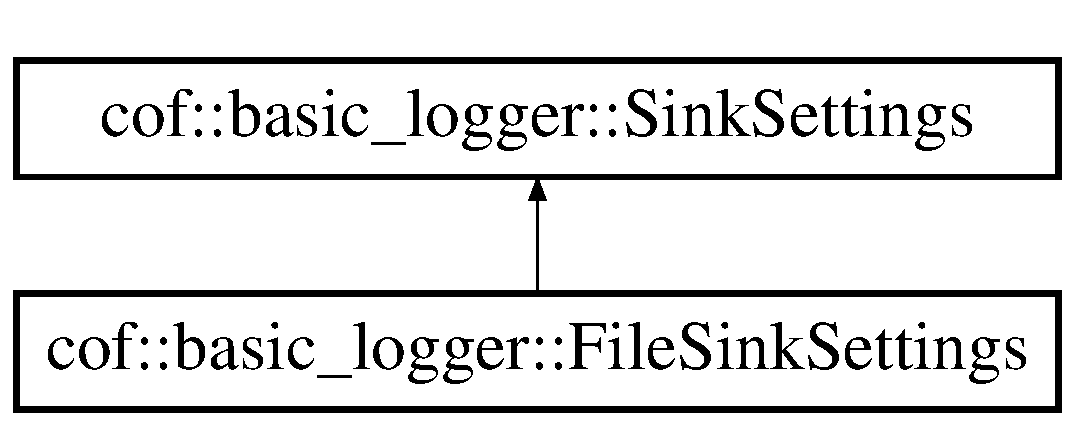
\includegraphics[height=2.000000cm]{structcof_1_1basic__logger_1_1_file_sink_settings}
\end{center}
\end{figure}
\subsection*{Public Member Functions}
\begin{DoxyCompactItemize}
\item 
\mbox{\Hypertarget{structcof_1_1basic__logger_1_1_file_sink_settings_abc2a4e9ac5fe20c21b7bf95684c6e2b3}\label{structcof_1_1basic__logger_1_1_file_sink_settings_abc2a4e9ac5fe20c21b7bf95684c6e2b3}} 
{\bfseries File\+Sink\+Settings} (const char $\ast$File\+Str)
\item 
\mbox{\Hypertarget{structcof_1_1basic__logger_1_1_file_sink_settings_a1cda01667d68b065091959015b13619a}\label{structcof_1_1basic__logger_1_1_file_sink_settings_a1cda01667d68b065091959015b13619a}} 
{\bfseries File\+Sink\+Settings} (\hyperlink{structcof_1_1basic__logger_1_1_file_sink_settings}{File\+Sink\+Settings} \&\&other) noexcept
\end{DoxyCompactItemize}
\subsection*{Public Attributes}
\begin{DoxyCompactItemize}
\item 
\mbox{\Hypertarget{structcof_1_1basic__logger_1_1_file_sink_settings_a67a672d20da69ca7b856f0af464651c8}\label{structcof_1_1basic__logger_1_1_file_sink_settings_a67a672d20da69ca7b856f0af464651c8}} 
std\+::string {\bfseries File\+Str} \{\}
\item 
\mbox{\Hypertarget{structcof_1_1basic__logger_1_1_file_sink_settings_a8c2e26cdb44227a7e77dfe7488bed7a0}\label{structcof_1_1basic__logger_1_1_file_sink_settings_a8c2e26cdb44227a7e77dfe7488bed7a0}} 
std\+::string {\bfseries File\+Mode} \{ \char`\"{}a+\char`\"{} \}
\end{DoxyCompactItemize}


\subsection{Detailed Description}
Defines settings for the \hyperlink{classcof_1_1basic__logger_1_1_file}{File} logger. 

Can set the logging file and its write more. Important for the I/O process. Default is {\ttfamily a+} append to an file. If not exists creates file.

\begin{DoxyAuthor}{Author}
Simon Renger 
\end{DoxyAuthor}
\begin{DoxyVersion}{Version}
1.\+0 
\end{DoxyVersion}
\begin{DoxyDate}{Date}
2018 
\end{DoxyDate}
\begin{DoxyCopyright}{Copyright}
The M\+IT License 
\end{DoxyCopyright}
\begin{Desc}
\item[Examples\+: ]\par
\hyperlink{example_freefunction_8cpp-example}{example\+\_\+freefunction.\+cpp}.\end{Desc}


The documentation for this struct was generated from the following file\+:\begin{DoxyCompactItemize}
\item 
A\+:/collectionofframeworks/\+Basic\+Logger/include/\+Sinks/\hyperlink{_file_8h}{File.\+h}\end{DoxyCompactItemize}

\hypertarget{classcof_1_1basic__logger_1_1_logger}{}\section{cof\+:\+:basic\+\_\+logger\+:\+:Logger Class Reference}
\label{classcof_1_1basic__logger_1_1_logger}\index{cof\+::basic\+\_\+logger\+::\+Logger@{cof\+::basic\+\_\+logger\+::\+Logger}}


A basic non multi threaded logger.  




{\ttfamily \#include $<$Basic\+Logger.\+h$>$}

\subsection*{Public Member Functions}
\begin{DoxyCompactItemize}
\item 
\mbox{\Hypertarget{classcof_1_1basic__logger_1_1_logger_a6eb22968894b3b6c344e0a1899cf447d}\label{classcof_1_1basic__logger_1_1_logger_a6eb22968894b3b6c344e0a1899cf447d}} 
{\bfseries Logger} (const \hyperlink{classcof_1_1basic__logger_1_1_logger}{Logger} \&other)=delete
\item 
\mbox{\Hypertarget{classcof_1_1basic__logger_1_1_logger_aa4d66cb63a0579fe8396e18d8bdbc058}\label{classcof_1_1basic__logger_1_1_logger_aa4d66cb63a0579fe8396e18d8bdbc058}} 
\hyperlink{classcof_1_1basic__logger_1_1_logger}{Logger} \& {\bfseries operator=} (const \hyperlink{classcof_1_1basic__logger_1_1_logger}{Logger} \&other)=delete
\item 
\mbox{\Hypertarget{classcof_1_1basic__logger_1_1_logger_ade6a4cfbf519c776bcebc3cd0cf1e240}\label{classcof_1_1basic__logger_1_1_logger_ade6a4cfbf519c776bcebc3cd0cf1e240}} 
{\bfseries Logger} (\hyperlink{classcof_1_1basic__logger_1_1_logger}{Logger} \&\&other) noexcept
\item 
\mbox{\Hypertarget{classcof_1_1basic__logger_1_1_logger_aa011d07c00035c9df2387589c88c02d8}\label{classcof_1_1basic__logger_1_1_logger_aa011d07c00035c9df2387589c88c02d8}} 
\hyperlink{classcof_1_1basic__logger_1_1_logger}{Logger} \& {\bfseries operator=} (\hyperlink{classcof_1_1basic__logger_1_1_logger}{Logger} \&\&other) noexcept
\item 
\mbox{\Hypertarget{classcof_1_1basic__logger_1_1_logger_a583530f90c7f07510bc89e9521180a05}\label{classcof_1_1basic__logger_1_1_logger_a583530f90c7f07510bc89e9521180a05}} 
{\bfseries Logger} (\hyperlink{classcof_1_1basic__logger_1_1_sink}{basic\+\_\+logger\+::\+Sink} $\ast$sink)
\item 
{\footnotesize template$<$typename... Args$>$ }\\void \hyperlink{classcof_1_1basic__logger_1_1_logger_a4c698d87cddfe754221f7657caa2b06a}{Log} (const char $\ast$form\+Str, const Args \&... args)
\begin{DoxyCompactList}\small\item\em Logging function. \end{DoxyCompactList}\item 
{\footnotesize template$<$typename... Args$>$ }\\void \hyperlink{classcof_1_1basic__logger_1_1_logger_ad518be9654acd1d698c6a8eb50262d52}{Warn} (const char $\ast$form\+Str, const Args \&... args)
\begin{DoxyCompactList}\small\item\em Logging function. \end{DoxyCompactList}\item 
{\footnotesize template$<$typename... Args$>$ }\\void \hyperlink{classcof_1_1basic__logger_1_1_logger_a4562cce09bb747a47ce052f5388b16b6}{Debug} (const char $\ast$form\+Str, const Args \&... args)
\begin{DoxyCompactList}\small\item\em Logging function. \end{DoxyCompactList}\item 
{\footnotesize template$<$typename... Args$>$ }\\void \hyperlink{classcof_1_1basic__logger_1_1_logger_a9a280522d90572bed5d06f7540d42522}{Info} (const char $\ast$form\+Str, const Args \&... args)
\begin{DoxyCompactList}\small\item\em Logging function. \end{DoxyCompactList}\item 
{\footnotesize template$<$typename... Args$>$ }\\void \hyperlink{classcof_1_1basic__logger_1_1_logger_a6de6aa4607ebb5edf8d3732f214f41f1}{Error} (const char $\ast$form\+Str, const Args \&... args)
\begin{DoxyCompactList}\small\item\em Logging function. \end{DoxyCompactList}\end{DoxyCompactItemize}
\subsection*{Private Attributes}
\begin{DoxyCompactItemize}
\item 
\mbox{\Hypertarget{classcof_1_1basic__logger_1_1_logger_a7972063db1d84fe2a5fb3e5fde1ad997}\label{classcof_1_1basic__logger_1_1_logger_a7972063db1d84fe2a5fb3e5fde1ad997}} 
std\+::unique\+\_\+ptr$<$ \hyperlink{classcof_1_1basic__logger_1_1_sink}{basic\+\_\+logger\+::\+Sink} $>$ {\bfseries sink\+\_\+}
\end{DoxyCompactItemize}


\subsection{Detailed Description}
A basic non multi threaded logger. 

This is the basic logger imnpl. See \href{https://github.com/fmtlib/fmt/}{\tt fmt} for more information of the formatting. {\bfseries This is a move only type.} \begin{DoxyAuthor}{Author}
Simon Renger 
\end{DoxyAuthor}
\begin{DoxyVersion}{Version}
1.\+0 
\end{DoxyVersion}
\begin{DoxyDate}{Date}
2018 
\end{DoxyDate}
\begin{DoxyPrecond}{Precondition}
If used outside of Debug mode the macro {\ttfamily C\+O\+F\+\_\+\+U\+S\+E\+\_\+\+L\+O\+G\+G\+ER} needs to be defined. Otherwise all functions/methods will leave a zero fingerprint. 
\end{DoxyPrecond}
\begin{DoxyWarning}{Warning}
Move only type. 
\end{DoxyWarning}
\hypertarget{classcof_1_1basic__logger_1_1_logger_example}{}\subsection{Example}\label{classcof_1_1basic__logger_1_1_logger_example}

\begin{DoxyCodeInclude}

\textcolor{preprocessor}{#include "\hyperlink{_logger_8h}{Logger.h}"}

\textcolor{keyword}{class }OtherClass
\{
\textcolor{keyword}{public}:
    \textcolor{keyword}{explicit} OtherClass(\hyperlink{classcof_1_1basic__logger_1_1_logger}{cof::basic\_logger::Logger}& logger);

    \textcolor{keywordtype}{void} some\_action();
\textcolor{keyword}{private}:
    \hyperlink{classcof_1_1basic__logger_1_1_logger}{cof::basic\_logger::Logger}& logger\_;
\};

OtherClass::OtherClass(\hyperlink{classcof_1_1basic__logger_1_1_logger}{cof::basic\_logger::Logger}& logger) : logger\_(logger)
\{
\}

\textcolor{keywordtype}{void} OtherClass::some\_action()
\{
    logger\_.Debug(\textcolor{stringliteral}{"I am doing something"});
\}

\textcolor{keyword}{class }Application
\{
\textcolor{keyword}{public}:
    Application(\hyperlink{classcof_1_1basic__logger_1_1_logger}{cof::basic\_logger::Logger}&& logger);
    \textcolor{keywordtype}{void} do\_something();
\textcolor{keyword}{private}:
    \hyperlink{classcof_1_1basic__logger_1_1_logger}{cof::basic\_logger::Logger} logger\_;
    OtherClass action\_;
\};

Application::Application(\hyperlink{classcof_1_1basic__logger_1_1_logger}{cof::basic\_logger::Logger}&& logger): logger\_(std::move(
      logger)), action\_(logger\_)
\{
\}

\textcolor{keywordtype}{void} Application::do\_something()
\{
    logger\_.Info(\textcolor{stringliteral}{"I am doing something"});
    action\_.some\_action();
\}



\textcolor{keywordtype}{int} main()
\{
    \textcolor{keyword}{auto}* sink = \textcolor{keyword}{new} \hyperlink{classcof_1_1basic__logger_1_1_std_out}{cof::basic\_logger::StdOut}(\textcolor{keyword}{new} 
      \hyperlink{structcof_1_1basic__logger_1_1_sink_settings}{cof::basic\_logger::SinkSettings});
    \textcolor{comment}{// takes the ownership of the pointer.}
    \textcolor{keyword}{auto} logger = \hyperlink{classcof_1_1basic__logger_1_1_logger}{cof::basic\_logger::Logger}(sink);

    Application app(std::move(logger));
    app.do\_something();

    \textcolor{keywordflow}{return} 0;
\}
\end{DoxyCodeInclude}
 \begin{Desc}
\item[Examples\+: ]\par
\hyperlink{example_object_8cpp-example}{example\+\_\+object.\+cpp}.\end{Desc}


\subsection{Member Function Documentation}
\mbox{\Hypertarget{classcof_1_1basic__logger_1_1_logger_a4562cce09bb747a47ce052f5388b16b6}\label{classcof_1_1basic__logger_1_1_logger_a4562cce09bb747a47ce052f5388b16b6}} 
\index{cof\+::basic\+\_\+logger\+::\+Logger@{cof\+::basic\+\_\+logger\+::\+Logger}!Debug@{Debug}}
\index{Debug@{Debug}!cof\+::basic\+\_\+logger\+::\+Logger@{cof\+::basic\+\_\+logger\+::\+Logger}}
\subsubsection{\texorpdfstring{Debug()}{Debug()}}
{\footnotesize\ttfamily template$<$typename... Args$>$ \\
void cof\+::basic\+\_\+logger\+::\+Logger\+::\+Debug (\begin{DoxyParamCaption}\item[{const char $\ast$}]{form\+Str,  }\item[{const Args \&...}]{args }\end{DoxyParamCaption})\hspace{0.3cm}{\ttfamily [inline]}}



Logging function. 


\begin{DoxyParams}{Parameters}
{\em form\+Str} & ftm style format. e.\+g. {\ttfamily User \#\+ID\{\} logged in at \{\}. with the IP\{\}} \\
\hline
{\em args} & Variadic arguments for the replacements. e.\+g. time etc. \\
\hline
\end{DoxyParams}

\begin{DoxyTemplParams}{Template Parameters}
{\em Args} & Variadic template argument important for the format replacements. \\
\hline
\end{DoxyTemplParams}
\begin{DoxySeeAlso}{See also}
\hyperlink{classcof_1_1basic__logger_1_1_sink_a085f8c690add00cf55ef0754c5900397}{cof\+::basic\+\_\+logger\+::\+Sink\+::\+Sink\+In()} for more information on the implementation of the actual logging 
\end{DoxySeeAlso}
\mbox{\Hypertarget{classcof_1_1basic__logger_1_1_logger_a6de6aa4607ebb5edf8d3732f214f41f1}\label{classcof_1_1basic__logger_1_1_logger_a6de6aa4607ebb5edf8d3732f214f41f1}} 
\index{cof\+::basic\+\_\+logger\+::\+Logger@{cof\+::basic\+\_\+logger\+::\+Logger}!Error@{Error}}
\index{Error@{Error}!cof\+::basic\+\_\+logger\+::\+Logger@{cof\+::basic\+\_\+logger\+::\+Logger}}
\subsubsection{\texorpdfstring{Error()}{Error()}}
{\footnotesize\ttfamily template$<$typename... Args$>$ \\
void cof\+::basic\+\_\+logger\+::\+Logger\+::\+Error (\begin{DoxyParamCaption}\item[{const char $\ast$}]{form\+Str,  }\item[{const Args \&...}]{args }\end{DoxyParamCaption})\hspace{0.3cm}{\ttfamily [inline]}}



Logging function. 


\begin{DoxyParams}{Parameters}
{\em form\+Str} & ftm style format. e.\+g. {\ttfamily User \#\+ID\{\} logged in at \{\}. with the IP\{\}} \\
\hline
{\em args} & Variadic arguments for the replacements. e.\+g. time etc. \\
\hline
\end{DoxyParams}

\begin{DoxyTemplParams}{Template Parameters}
{\em Args} & Variadic template argument important for the format replacements. \\
\hline
\end{DoxyTemplParams}
\begin{DoxySeeAlso}{See also}
\hyperlink{classcof_1_1basic__logger_1_1_sink_a085f8c690add00cf55ef0754c5900397}{cof\+::basic\+\_\+logger\+::\+Sink\+::\+Sink\+In()} for more information on the implementation of the actual logging 
\end{DoxySeeAlso}
\mbox{\Hypertarget{classcof_1_1basic__logger_1_1_logger_a9a280522d90572bed5d06f7540d42522}\label{classcof_1_1basic__logger_1_1_logger_a9a280522d90572bed5d06f7540d42522}} 
\index{cof\+::basic\+\_\+logger\+::\+Logger@{cof\+::basic\+\_\+logger\+::\+Logger}!Info@{Info}}
\index{Info@{Info}!cof\+::basic\+\_\+logger\+::\+Logger@{cof\+::basic\+\_\+logger\+::\+Logger}}
\subsubsection{\texorpdfstring{Info()}{Info()}}
{\footnotesize\ttfamily template$<$typename... Args$>$ \\
void cof\+::basic\+\_\+logger\+::\+Logger\+::\+Info (\begin{DoxyParamCaption}\item[{const char $\ast$}]{form\+Str,  }\item[{const Args \&...}]{args }\end{DoxyParamCaption})\hspace{0.3cm}{\ttfamily [inline]}}



Logging function. 


\begin{DoxyParams}{Parameters}
{\em form\+Str} & ftm style format. e.\+g. {\ttfamily User \#\+ID\{\} logged in at \{\}. with the IP\{\}} \\
\hline
{\em args} & Variadic arguments for the replacements. e.\+g. time etc. \\
\hline
\end{DoxyParams}

\begin{DoxyTemplParams}{Template Parameters}
{\em Args} & Variadic template argument important for the format replacements. \\
\hline
\end{DoxyTemplParams}
\begin{DoxySeeAlso}{See also}
\hyperlink{classcof_1_1basic__logger_1_1_sink_a085f8c690add00cf55ef0754c5900397}{cof\+::basic\+\_\+logger\+::\+Sink\+::\+Sink\+In()} for more information on the implementation of the actual logging 
\end{DoxySeeAlso}
\mbox{\Hypertarget{classcof_1_1basic__logger_1_1_logger_a4c698d87cddfe754221f7657caa2b06a}\label{classcof_1_1basic__logger_1_1_logger_a4c698d87cddfe754221f7657caa2b06a}} 
\index{cof\+::basic\+\_\+logger\+::\+Logger@{cof\+::basic\+\_\+logger\+::\+Logger}!Log@{Log}}
\index{Log@{Log}!cof\+::basic\+\_\+logger\+::\+Logger@{cof\+::basic\+\_\+logger\+::\+Logger}}
\subsubsection{\texorpdfstring{Log()}{Log()}}
{\footnotesize\ttfamily template$<$typename... Args$>$ \\
void cof\+::basic\+\_\+logger\+::\+Logger\+::\+Log (\begin{DoxyParamCaption}\item[{const char $\ast$}]{form\+Str,  }\item[{const Args \&...}]{args }\end{DoxyParamCaption})\hspace{0.3cm}{\ttfamily [inline]}}



Logging function. 


\begin{DoxyParams}{Parameters}
{\em form\+Str} & ftm style format. e.\+g. {\ttfamily User \#\+ID\{\} logged in at \{\}. with the IP\{\}} \\
\hline
{\em args} & Variadic arguments for the replacements. e.\+g. time etc. \\
\hline
\end{DoxyParams}

\begin{DoxyTemplParams}{Template Parameters}
{\em Args} & Variadic template argument important for the format replacements. \\
\hline
\end{DoxyTemplParams}
\begin{DoxySeeAlso}{See also}
\hyperlink{classcof_1_1basic__logger_1_1_sink_a085f8c690add00cf55ef0754c5900397}{cof\+::basic\+\_\+logger\+::\+Sink\+::\+Sink\+In()} for more information on the implementation of the actual logging 
\end{DoxySeeAlso}
\mbox{\Hypertarget{classcof_1_1basic__logger_1_1_logger_ad518be9654acd1d698c6a8eb50262d52}\label{classcof_1_1basic__logger_1_1_logger_ad518be9654acd1d698c6a8eb50262d52}} 
\index{cof\+::basic\+\_\+logger\+::\+Logger@{cof\+::basic\+\_\+logger\+::\+Logger}!Warn@{Warn}}
\index{Warn@{Warn}!cof\+::basic\+\_\+logger\+::\+Logger@{cof\+::basic\+\_\+logger\+::\+Logger}}
\subsubsection{\texorpdfstring{Warn()}{Warn()}}
{\footnotesize\ttfamily template$<$typename... Args$>$ \\
void cof\+::basic\+\_\+logger\+::\+Logger\+::\+Warn (\begin{DoxyParamCaption}\item[{const char $\ast$}]{form\+Str,  }\item[{const Args \&...}]{args }\end{DoxyParamCaption})\hspace{0.3cm}{\ttfamily [inline]}}



Logging function. 


\begin{DoxyParams}{Parameters}
{\em form\+Str} & ftm style format. e.\+g. {\ttfamily User \#\+ID\{\} logged in at \{\}. with the IP\{\}} \\
\hline
{\em args} & Variadic arguments for the replacements. e.\+g. time etc. \\
\hline
\end{DoxyParams}

\begin{DoxyTemplParams}{Template Parameters}
{\em Args} & Variadic template argument important for the format replacements. \\
\hline
\end{DoxyTemplParams}
\begin{DoxySeeAlso}{See also}
\hyperlink{classcof_1_1basic__logger_1_1_sink_a085f8c690add00cf55ef0754c5900397}{cof\+::basic\+\_\+logger\+::\+Sink\+::\+Sink\+In()} for more information on the implementation of the actual logging 
\end{DoxySeeAlso}


The documentation for this class was generated from the following file\+:\begin{DoxyCompactItemize}
\item 
A\+:/collectionofframeworks/\+Basic\+Logger/include/\hyperlink{_basic_logger_8h}{Basic\+Logger.\+h}\end{DoxyCompactItemize}

\hypertarget{classcof_1_1basic__logger_1_1_sink}{}\section{cof\+:\+:basic\+\_\+logger\+:\+:Sink Class Reference}
\label{classcof_1_1basic__logger_1_1_sink}\index{cof\+::basic\+\_\+logger\+::\+Sink@{cof\+::basic\+\_\+logger\+::\+Sink}}


The Base \hyperlink{classcof_1_1basic__logger_1_1_sink}{Sink} class.  




{\ttfamily \#include $<$Sink.\+h$>$}

Inheritance diagram for cof\+:\+:basic\+\_\+logger\+:\+:Sink\+:\begin{figure}[H]
\begin{center}
\leavevmode
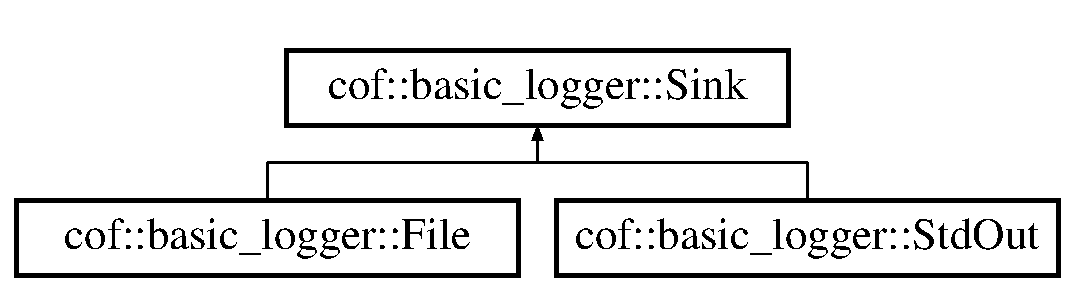
\includegraphics[height=2.000000cm]{classcof_1_1basic__logger_1_1_sink}
\end{center}
\end{figure}
\subsection*{Public Member Functions}
\begin{DoxyCompactItemize}
\item 
void \hyperlink{classcof_1_1basic__logger_1_1_sink_a085f8c690add00cf55ef0754c5900397}{Sink\+In} (Level lvl, std\+::string \&\&message)
\begin{DoxyCompactList}\small\item\em format data \end{DoxyCompactList}\end{DoxyCompactItemize}
\subsection*{Protected Member Functions}
\begin{DoxyCompactItemize}
\item 
\mbox{\Hypertarget{classcof_1_1basic__logger_1_1_sink_aa95b0d438e4561464ba80ba3312a7ff4}\label{classcof_1_1basic__logger_1_1_sink_aa95b0d438e4561464ba80ba3312a7ff4}} 
virtual void {\bfseries Process} (Level lvl, fmt\+::memory\+\_\+buffer \&\&message)=0
\item 
\mbox{\Hypertarget{classcof_1_1basic__logger_1_1_sink_aff876363f1ab16500c493c834f726015}\label{classcof_1_1basic__logger_1_1_sink_aff876363f1ab16500c493c834f726015}} 
std\+::string {\bfseries Get\+Formatted\+Date} ()
\end{DoxyCompactItemize}
\subsection*{Protected Attributes}
\begin{DoxyCompactItemize}
\item 
\mbox{\Hypertarget{classcof_1_1basic__logger_1_1_sink_a8befddc7ae7d03530bc059a3173715ef}\label{classcof_1_1basic__logger_1_1_sink_a8befddc7ae7d03530bc059a3173715ef}} 
std\+::array$<$ const char $\ast$, 5 $>$ {\bfseries levels\+\_\+} \{\char`\"{}L\+OG\char`\"{}, \char`\"{}I\+N\+FO\char`\"{}, \char`\"{}D\+E\+B\+UG\char`\"{}, \char`\"{}E\+R\+R\+OR\char`\"{}, \char`\"{}W\+A\+RN\char`\"{}\}
\end{DoxyCompactItemize}


\subsection{Detailed Description}
The Base \hyperlink{classcof_1_1basic__logger_1_1_sink}{Sink} class. 

\begin{DoxyAuthor}{Author}
Simon Renger
\end{DoxyAuthor}
\begin{DoxyVersion}{Version}
1.\+0 
\end{DoxyVersion}
\begin{DoxyDate}{Date}
2018 
\end{DoxyDate}
\begin{DoxyCopyright}{Copyright}
The M\+IT License 
\end{DoxyCopyright}
\begin{DoxySeeAlso}{See also}
\href{https://github.com/fmtlib/fmt/}{\tt fmt fmt\+::memory\+\_\+buffer} 
\end{DoxySeeAlso}


\subsection{Member Function Documentation}
\mbox{\Hypertarget{classcof_1_1basic__logger_1_1_sink_a085f8c690add00cf55ef0754c5900397}\label{classcof_1_1basic__logger_1_1_sink_a085f8c690add00cf55ef0754c5900397}} 
\index{cof\+::basic\+\_\+logger\+::\+Sink@{cof\+::basic\+\_\+logger\+::\+Sink}!Sink\+In@{Sink\+In}}
\index{Sink\+In@{Sink\+In}!cof\+::basic\+\_\+logger\+::\+Sink@{cof\+::basic\+\_\+logger\+::\+Sink}}
\subsubsection{\texorpdfstring{Sink\+In()}{SinkIn()}}
{\footnotesize\ttfamily void cof\+::basic\+\_\+logger\+::\+Sink\+::\+Sink\+In (\begin{DoxyParamCaption}\item[{Level}]{lvl,  }\item[{std\+::string \&\&}]{message }\end{DoxyParamCaption})}



format data 

Uses fmt to format content. Adds the Date as well as the log level to the message. Calls internally {\ttfamily Process}. \begin{DoxyAuthor}{Author}
Simon Renger 
\end{DoxyAuthor}
\begin{DoxyVersion}{Version}
1.\+0 
\end{DoxyVersion}
\begin{DoxyDate}{Date}
2018 
\end{DoxyDate}
\begin{DoxyCopyright}{Copyright}
The M\+IT License 
\end{DoxyCopyright}


The documentation for this class was generated from the following files\+:\begin{DoxyCompactItemize}
\item 
A\+:/collectionofframeworks/\+Basic\+Logger/include/\+Sinks/\hyperlink{_sink_8h}{Sink.\+h}\item 
A\+:/collectionofframeworks/\+Basic\+Logger/src/\+Sinks/Sink.\+cpp\end{DoxyCompactItemize}

\hypertarget{structcof_1_1basic__logger_1_1_sink_settings}{}\section{cof\+:\+:basic\+\_\+logger\+:\+:Sink\+Settings Struct Reference}
\label{structcof_1_1basic__logger_1_1_sink_settings}\index{cof\+::basic\+\_\+logger\+::\+Sink\+Settings@{cof\+::basic\+\_\+logger\+::\+Sink\+Settings}}


The Base \hyperlink{structcof_1_1basic__logger_1_1_sink_settings}{Sink\+Settings} class.  




{\ttfamily \#include $<$Sink.\+h$>$}

Inheritance diagram for cof\+:\+:basic\+\_\+logger\+:\+:Sink\+Settings\+:\begin{figure}[H]
\begin{center}
\leavevmode
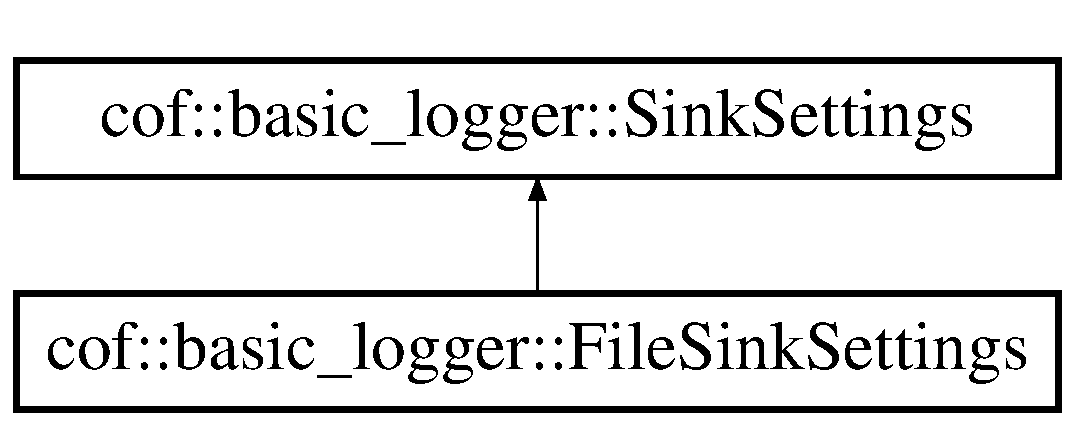
\includegraphics[height=2.000000cm]{structcof_1_1basic__logger_1_1_sink_settings}
\end{center}
\end{figure}
\subsection*{Public Member Functions}
\begin{DoxyCompactItemize}
\item 
\mbox{\Hypertarget{structcof_1_1basic__logger_1_1_sink_settings_a34768fcf9b8f2057c2a6c19c5d6aa002}\label{structcof_1_1basic__logger_1_1_sink_settings_a34768fcf9b8f2057c2a6c19c5d6aa002}} 
{\bfseries Sink\+Settings} (\hyperlink{structcof_1_1basic__logger_1_1_sink_settings}{Sink\+Settings} \&\&other) noexcept
\end{DoxyCompactItemize}


\subsection{Detailed Description}
The Base \hyperlink{structcof_1_1basic__logger_1_1_sink_settings}{Sink\+Settings} class. 

can be used to send extra information to the \hyperlink{classcof_1_1basic__logger_1_1_sink}{Sink}.

\begin{DoxyAuthor}{Author}
Simon Renger 
\end{DoxyAuthor}
\begin{DoxyVersion}{Version}
1.\+0 
\end{DoxyVersion}
\begin{DoxyDate}{Date}
2018 
\end{DoxyDate}
\begin{DoxyCopyright}{Copyright}
The M\+IT License 
\end{DoxyCopyright}
\begin{Desc}
\item[Examples\+: ]\par
\hyperlink{example_freefunction_8cpp-example}{example\+\_\+freefunction.\+cpp}, and \hyperlink{example_object_8cpp-example}{example\+\_\+object.\+cpp}.\end{Desc}


The documentation for this struct was generated from the following file\+:\begin{DoxyCompactItemize}
\item 
A\+:/collectionofframeworks/\+Basic\+Logger/include/\+Sinks/\hyperlink{_sink_8h}{Sink.\+h}\end{DoxyCompactItemize}

\hypertarget{classcof_1_1basic__logger_1_1_std_out}{}\section{cof\+:\+:basic\+\_\+logger\+:\+:Std\+Out Class Reference}
\label{classcof_1_1basic__logger_1_1_std_out}\index{cof\+::basic\+\_\+logger\+::\+Std\+Out@{cof\+::basic\+\_\+logger\+::\+Std\+Out}}


Terminal logging.  




{\ttfamily \#include $<$Std\+Out.\+h$>$}

Inheritance diagram for cof\+:\+:basic\+\_\+logger\+:\+:Std\+Out\+:\begin{figure}[H]
\begin{center}
\leavevmode
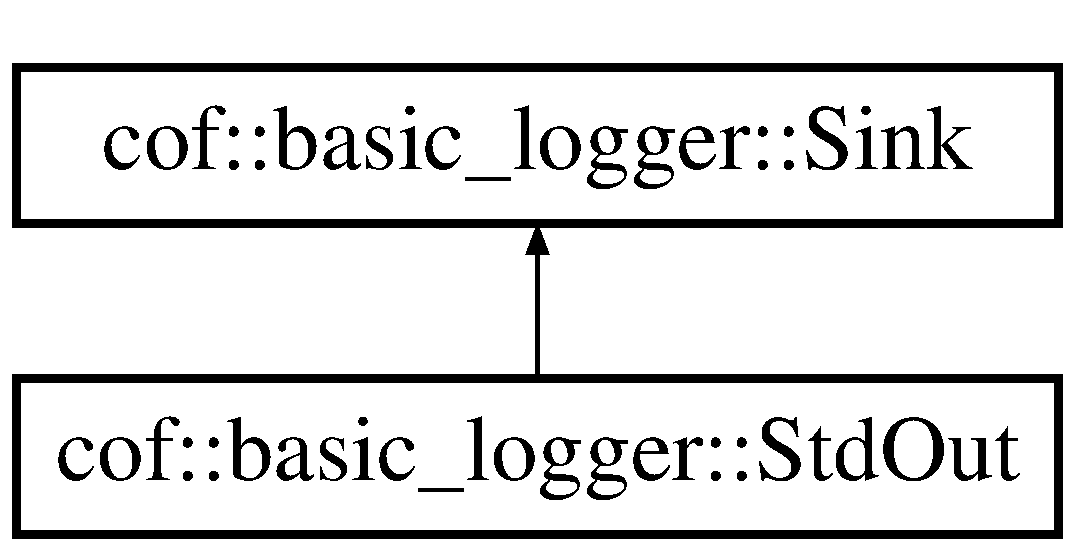
\includegraphics[height=2.000000cm]{classcof_1_1basic__logger_1_1_std_out}
\end{center}
\end{figure}
\subsection*{Public Member Functions}
\begin{DoxyCompactItemize}
\item 
\mbox{\Hypertarget{classcof_1_1basic__logger_1_1_std_out_a2943366adfadbfeb31bb7126b4c710ae}\label{classcof_1_1basic__logger_1_1_std_out_a2943366adfadbfeb31bb7126b4c710ae}} 
{\bfseries Std\+Out} (\hyperlink{structcof_1_1basic__logger_1_1_sink_settings}{Sink\+Settings} $\ast$settings)
\end{DoxyCompactItemize}
\subsection*{Protected Member Functions}
\begin{DoxyCompactItemize}
\item 
\mbox{\Hypertarget{classcof_1_1basic__logger_1_1_std_out_a75cb54e45babb7991d57199e12f1f338}\label{classcof_1_1basic__logger_1_1_std_out_a75cb54e45babb7991d57199e12f1f338}} 
void \hyperlink{classcof_1_1basic__logger_1_1_std_out_a75cb54e45babb7991d57199e12f1f338}{Process} (Level lvl, fmt\+::memory\+\_\+buffer \&\&message) override
\begin{DoxyCompactList}\small\item\em Uses {\ttfamily fwrite} and {\ttfamily fflush} \end{DoxyCompactList}\end{DoxyCompactItemize}
\subsection*{Additional Inherited Members}


\subsection{Detailed Description}
Terminal logging. 

Loggs with {\ttfamily stdout} to the terminal unless the log level is {\ttfamily Level\+::\+E\+R\+R\+OR} then it is using {\ttfamily stderr}.

\begin{DoxyAuthor}{Author}
Simon Renger 
\end{DoxyAuthor}
\begin{DoxyVersion}{Version}
1.\+0 
\end{DoxyVersion}
\begin{DoxyDate}{Date}
2018 
\end{DoxyDate}
\begin{DoxyCopyright}{Copyright}
The M\+IT License 
\end{DoxyCopyright}
\begin{Desc}
\item[Examples\+: ]\par
\hyperlink{example_object_8cpp-example}{example\+\_\+object.\+cpp}.\end{Desc}


The documentation for this class was generated from the following files\+:\begin{DoxyCompactItemize}
\item 
A\+:/collectionofframeworks/\+Basic\+Logger/include/\+Sinks/\hyperlink{_std_out_8h}{Std\+Out.\+h}\item 
A\+:/collectionofframeworks/\+Basic\+Logger/src/\+Sinks/Std\+Out.\+cpp\end{DoxyCompactItemize}

\chapter{File Documentation}
\hypertarget{_basic_logger_8h}{}\section{A\+:/collectionofframeworks/\+Basic\+Logger/include/\+Basic\+Logger.h File Reference}
\label{_basic_logger_8h}\index{A\+:/collectionofframeworks/\+Basic\+Logger/include/\+Basic\+Logger.\+h@{A\+:/collectionofframeworks/\+Basic\+Logger/include/\+Basic\+Logger.\+h}}


Contains the basic impl of the logger class.  


{\ttfamily \#include \char`\"{}Sinks/\+Sink.\+h\char`\"{}}\newline
{\ttfamily \#include \char`\"{}fmt/format.\+h\char`\"{}}\newline
{\ttfamily \#include $<$string$>$}\newline
{\ttfamily \#include $<$memory$>$}\newline
\subsection*{Classes}
\begin{DoxyCompactItemize}
\item 
class \hyperlink{classcof_1_1basic__logger_1_1_logger}{cof\+::basic\+\_\+logger\+::\+Logger}
\begin{DoxyCompactList}\small\item\em A basic non multi threaded logger. \end{DoxyCompactList}\end{DoxyCompactItemize}


\subsection{Detailed Description}
Contains the basic impl of the logger class. 

see class description 
\hypertarget{_logger_8h}{}\section{A\+:/collectionofframeworks/\+Basic\+Logger/include/\+Logger.h File Reference}
\label{_logger_8h}\index{A\+:/collectionofframeworks/\+Basic\+Logger/include/\+Logger.\+h@{A\+:/collectionofframeworks/\+Basic\+Logger/include/\+Logger.\+h}}


Easy to include file.  


{\ttfamily \#include \char`\"{}Logging\+Function.\+h\char`\"{}}\newline
{\ttfamily \#include \char`\"{}Logging\+Macros.\+h\char`\"{}}\newline
{\ttfamily \#include \char`\"{}Sinks/\+File.\+h\char`\"{}}\newline
{\ttfamily \#include \char`\"{}Sinks/\+Std\+Out.\+h\char`\"{}}\newline


\subsection{Detailed Description}
Easy to include file. 

\begin{DoxyAuthor}{Author}
Simon Renger 
\end{DoxyAuthor}
\begin{DoxyVersion}{Version}
1.\+0 
\end{DoxyVersion}
\begin{DoxyDate}{Date}
2018 
\end{DoxyDate}
\begin{DoxyCopyright}{Copyright}
The M\+IT License 
\end{DoxyCopyright}
\hypertarget{_logger_8h_Examples}{}\subsection{Examples}\label{_logger_8h_Examples}
\hypertarget{_logger_8h_example_object}{}\subsubsection{Object Approach}\label{_logger_8h_example_object}

\begin{DoxyCodeInclude}

\textcolor{preprocessor}{#include "\hyperlink{_logger_8h}{Logger.h}"}

\textcolor{keyword}{class }OtherClass
\{
\textcolor{keyword}{public}:
    \textcolor{keyword}{explicit} OtherClass(\hyperlink{classcof_1_1basic__logger_1_1_logger}{cof::basic\_logger::Logger}& logger);

    \textcolor{keywordtype}{void} some\_action();
\textcolor{keyword}{private}:
    \hyperlink{classcof_1_1basic__logger_1_1_logger}{cof::basic\_logger::Logger}& logger\_;
\};

OtherClass::OtherClass(\hyperlink{classcof_1_1basic__logger_1_1_logger}{cof::basic\_logger::Logger}& logger) : logger\_(logger)
\{
\}

\textcolor{keywordtype}{void} OtherClass::some\_action()
\{
    logger\_.Debug(\textcolor{stringliteral}{"I am doing something"});
\}

\textcolor{keyword}{class }Application
\{
\textcolor{keyword}{public}:
    Application(\hyperlink{classcof_1_1basic__logger_1_1_logger}{cof::basic\_logger::Logger}&& logger);
    \textcolor{keywordtype}{void} do\_something();
\textcolor{keyword}{private}:
    \hyperlink{classcof_1_1basic__logger_1_1_logger}{cof::basic\_logger::Logger} logger\_;
    OtherClass action\_;
\};

Application::Application(\hyperlink{classcof_1_1basic__logger_1_1_logger}{cof::basic\_logger::Logger}&& logger): logger\_(std::move(
      logger)), action\_(logger\_)
\{
\}

\textcolor{keywordtype}{void} Application::do\_something()
\{
    logger\_.Info(\textcolor{stringliteral}{"I am doing something"});
    action\_.some\_action();
\}



\textcolor{keywordtype}{int} main()
\{
    \textcolor{keyword}{auto}* sink = \textcolor{keyword}{new} \hyperlink{classcof_1_1basic__logger_1_1_std_out}{cof::basic\_logger::StdOut}(\textcolor{keyword}{new} 
      \hyperlink{structcof_1_1basic__logger_1_1_sink_settings}{cof::basic\_logger::SinkSettings});
    \textcolor{comment}{// takes the ownership of the pointer.}
    \textcolor{keyword}{auto} logger = \hyperlink{classcof_1_1basic__logger_1_1_logger}{cof::basic\_logger::Logger}(sink);

    Application app(std::move(logger));
    app.do\_something();

    \textcolor{keywordflow}{return} 0;
\}
\end{DoxyCodeInclude}
 \hypertarget{_logger_8h_example_macro}{}\subsubsection{Macro Approach}\label{_logger_8h_example_macro}

\begin{DoxyCodeInclude}

\textcolor{preprocessor}{#include "\hyperlink{_logger_8h}{Logger.h}"}

\textcolor{keywordtype}{int} main()
\{
    LOGGER\_INIT\_STDOUT()
    \hyperlink{_logging_macros_8h_a018a1fe4b078f1a684610657a5848860}{LOG}("Macro Log Message")
    \hyperlink{_logging_macros_8h_a5dd0aa9e28b0c7db286181cfc81ebb94}{WARN}("Macro Warn Message")
    \hyperlink{_logging_macros_8h_aafc148cee6d6c9e76b4ef417c7056f8f}{INFO}("Macro Info Message")
    \hyperlink{_logging_macros_8h_a614c336056da6e8a7e6a06ed991b9feb}{DEBUG}("Macro Debug Message")
    \hyperlink{_logging_macros_8h_a78e40dfd87f516e322340d249027aea1}{ERROR}("Macro Error Message")
    \hyperlink{_logging_macros_8h_a949408ae41659956042cdbe1e59281f3}{LOGGER\_DEINIT}

    return 0;
\}
\end{DoxyCodeInclude}
 \hypertarget{_logger_8h_example_freefunctions}{}\subsubsection{Freefunctions Approach}\label{_logger_8h_example_freefunctions}

\begin{DoxyCodeInclude}
\textcolor{preprocessor}{#include "\hyperlink{_logger_8h}{Logger.h}"}
\textcolor{keywordtype}{int} main()
\{
    cof::basic\_logger::Init<cof::basic\_logger::StdOut>(std::move(
      \hyperlink{structcof_1_1basic__logger_1_1_sink_settings}{cof::basic\_logger::SinkSettings}\{\}));
    \hyperlink{_logging_function_8h_a1f56bcf4dd7901f39b3386261c75d4a5}{cof::Log}(\textcolor{stringliteral}{"Free function Log Message"});
    \hyperlink{_logging_function_8h_ac0c0af18a99bcd635fb89679890cdeaa}{cof::Warn}(\textcolor{stringliteral}{"Free function Warn Message"});
    \hyperlink{_logging_function_8h_a4d2fa4bc5cade7fdb692a0615b489997}{cof::Info}(\textcolor{stringliteral}{"Free function Info Message"});
    \hyperlink{_logging_function_8h_ac0fff05470889b9bf801966564dddb36}{cof::Debug}(\textcolor{stringliteral}{"Free function Debug Message"});
    \hyperlink{_logging_function_8h_a09fbfa2e340f6dff1804c2a19a7b34f4}{cof::Error}(\textcolor{stringliteral}{"Free function Error Message"});
    cof::basic\_logger::Deint();

    \textcolor{keywordflow}{return} 0;
\}
\end{DoxyCodeInclude}
\hypertarget{_logger_8h_example_easyfunc_stdout}{}\paragraph{Easy to use initialization function for `stdout`}\label{_logger_8h_example_easyfunc_stdout}

\begin{DoxyCodeInclude}
\textcolor{preprocessor}{#include "\hyperlink{_logger_8h}{Logger.h}"}
\textcolor{keywordtype}{int} main()
\{
    cof::basic\_logger::InitStdOut();
    \hyperlink{_logging_function_8h_a1f56bcf4dd7901f39b3386261c75d4a5}{cof::Log}(\textcolor{stringliteral}{"Free function Log Message"});
    \hyperlink{_logging_function_8h_ac0c0af18a99bcd635fb89679890cdeaa}{cof::Warn}(\textcolor{stringliteral}{"Free function Warn Message"});
    \hyperlink{_logging_function_8h_a4d2fa4bc5cade7fdb692a0615b489997}{cof::Info}(\textcolor{stringliteral}{"Free function Info Message"});
    \hyperlink{_logging_function_8h_ac0fff05470889b9bf801966564dddb36}{cof::Debug}(\textcolor{stringliteral}{"Free function Debug Message"});
    \hyperlink{_logging_function_8h_a09fbfa2e340f6dff1804c2a19a7b34f4}{cof::Error}(\textcolor{stringliteral}{"Free function Error Message"});
    cof::basic\_logger::Deint();

    \textcolor{keywordflow}{return} 0;
\}
\end{DoxyCodeInclude}
\hypertarget{_logger_8h_example_easyfunc_file}{}\paragraph{Easy to use initialization function for `file`}\label{_logger_8h_example_easyfunc_file}

\begin{DoxyCodeInclude}
\textcolor{preprocessor}{#include "\hyperlink{_logger_8h}{Logger.h}"}
\textcolor{keywordtype}{int} main()
\{
    cof::basic\_logger::InitFile(\hyperlink{structcof_1_1basic__logger_1_1_file_sink_settings}{cof::basic\_logger::FileSinkSettings}\{ \textcolor{stringliteral}{"
      log.txt"} \});
    \hyperlink{_logging_function_8h_a1f56bcf4dd7901f39b3386261c75d4a5}{cof::Log}(\textcolor{stringliteral}{"Free function Log Message"});
    \hyperlink{_logging_function_8h_ac0c0af18a99bcd635fb89679890cdeaa}{cof::Warn}(\textcolor{stringliteral}{"Free function Warn Message"});
    \hyperlink{_logging_function_8h_a4d2fa4bc5cade7fdb692a0615b489997}{cof::Info}(\textcolor{stringliteral}{"Free function Info Message"});
    \hyperlink{_logging_function_8h_ac0fff05470889b9bf801966564dddb36}{cof::Debug}(\textcolor{stringliteral}{"Free function Debug Message"});
    \hyperlink{_logging_function_8h_a09fbfa2e340f6dff1804c2a19a7b34f4}{cof::Error}(\textcolor{stringliteral}{"Free function Error Message"});
    cof::basic\_logger::Deint();

    \textcolor{keywordflow}{return} 0;
\}
\end{DoxyCodeInclude}
 The M\+IT License

Copyright (c) 2018 Simon Renger, \href{https://simonrenger.de}{\tt https\+://simonrenger.\+de}

Permission is hereby granted, free of charge, to any person obtaining a copy of this software and associated documentation files (the \char`\"{}\+Software\char`\"{}), to deal in the Software without restriction, including without limitation the rights to use, copy, modify, merge, publish, distribute, sublicense, and/or sell copies of the Software, and to permit persons to whom the Software is furnished to do so, subject to the following conditions\+:

The above copyright notice and this permission notice shall be included in all copies or substantial portions of the Software.

T\+HE S\+O\+F\+T\+W\+A\+RE IS P\+R\+O\+V\+I\+D\+ED \char`\"{}\+A\+S I\+S\char`\"{}, W\+I\+T\+H\+O\+UT W\+A\+R\+R\+A\+N\+TY OF A\+NY K\+I\+ND, E\+X\+P\+R\+E\+SS OR I\+M\+P\+L\+I\+ED, I\+N\+C\+L\+U\+D\+I\+NG B\+UT N\+OT L\+I\+M\+I\+T\+ED TO T\+HE W\+A\+R\+R\+A\+N\+T\+I\+ES OF M\+E\+R\+C\+H\+A\+N\+T\+A\+B\+I\+L\+I\+TY, F\+I\+T\+N\+E\+SS F\+OR A P\+A\+R\+T\+I\+C\+U\+L\+AR P\+U\+R\+P\+O\+SE A\+ND N\+O\+N\+I\+N\+F\+R\+I\+N\+G\+E\+M\+E\+NT. IN NO E\+V\+E\+NT S\+H\+A\+LL T\+HE A\+U\+T\+H\+O\+RS OR C\+O\+P\+Y\+R\+I\+G\+HT H\+O\+L\+D\+E\+RS BE L\+I\+A\+B\+LE F\+OR A\+NY C\+L\+A\+IM, D\+A\+M\+A\+G\+ES OR O\+T\+H\+ER L\+I\+A\+B\+I\+L\+I\+TY, W\+H\+E\+T\+H\+ER IN AN A\+C\+T\+I\+ON OF C\+O\+N\+T\+R\+A\+CT, T\+O\+RT OR O\+T\+H\+E\+R\+W\+I\+SE, A\+R\+I\+S\+I\+NG F\+R\+OM, O\+UT OF OR IN C\+O\+N\+N\+E\+C\+T\+I\+ON W\+I\+TH T\+HE S\+O\+F\+T\+W\+A\+RE OR T\+HE U\+SE OR O\+T\+H\+ER D\+E\+A\+L\+I\+N\+GS IN T\+HE S\+O\+F\+T\+W\+A\+RE. 
\hypertarget{_logging_function_8h}{}\section{A\+:/collectionofframeworks/\+Basic\+Logger/include/\+Logging\+Function.h File Reference}
\label{_logging_function_8h}\index{A\+:/collectionofframeworks/\+Basic\+Logger/include/\+Logging\+Function.\+h@{A\+:/collectionofframeworks/\+Basic\+Logger/include/\+Logging\+Function.\+h}}


A collection of logging free functions.  


{\ttfamily \#include $<$cassert$>$}\newline
{\ttfamily \#include $<$type\+\_\+traits$>$}\newline
{\ttfamily \#include \char`\"{}Basic\+Logger.\+h\char`\"{}}\newline
\subsection*{Macros}
\begin{DoxyCompactItemize}
\item 
\#define \hyperlink{_logging_function_8h_a615f95e512a47e9a6f589a981120c6d2}{C\+O\+F\+\_\+\+C\+H\+E\+C\+K\+\_\+\+I\+F\+\_\+\+L\+O\+G\+G\+E\+R\+\_\+\+I\+S\+\_\+\+V\+A\+L\+ID}()
\begin{DoxyCompactList}\small\item\em check if logger is initialized if not runtime assert! \end{DoxyCompactList}\end{DoxyCompactItemize}
\subsection*{Functions}
\begin{DoxyCompactItemize}
\item 
{\footnotesize template$<$typename S , typename SS $>$ }\\void \hyperlink{_logging_function_8h_a7da3a6483f1a37634cdd72a2d111bc66}{cof\+::basic\+\_\+logger\+::\+Init} (SS \&\&settings)
\begin{DoxyCompactList}\small\item\em Initialization function. \end{DoxyCompactList}\item 
\mbox{\Hypertarget{_logging_function_8h_a4012911ebfed4e8a71c7abf0d5db7482}\label{_logging_function_8h_a4012911ebfed4e8a71c7abf0d5db7482}} 
void {\bfseries cof\+::basic\+\_\+logger\+::\+Init\+Std\+Out} ()
\item 
\mbox{\Hypertarget{_logging_function_8h_aca86de68e184d7bb4512126873aeb981}\label{_logging_function_8h_aca86de68e184d7bb4512126873aeb981}} 
void {\bfseries cof\+::basic\+\_\+logger\+::\+Init\+File} (\hyperlink{structcof_1_1basic__logger_1_1_file_sink_settings}{cof\+::basic\+\_\+logger\+::\+File\+Sink\+Settings} \&\&settings)
\item 
\mbox{\Hypertarget{_logging_function_8h_ae8eef673c2f017d2700cc936a3a1ba3d}\label{_logging_function_8h_ae8eef673c2f017d2700cc936a3a1ba3d}} 
void {\bfseries cof\+::basic\+\_\+logger\+::\+Deint} ()
\item 
{\footnotesize template$<$typename... Args$>$ }\\void \hyperlink{_logging_function_8h_a1f56bcf4dd7901f39b3386261c75d4a5}{cof\+::\+Log} (const char $\ast$format, const Args \&... args)
\begin{DoxyCompactList}\small\item\em Logging function. \end{DoxyCompactList}\item 
{\footnotesize template$<$typename... Args$>$ }\\void \hyperlink{_logging_function_8h_ac0fff05470889b9bf801966564dddb36}{cof\+::\+Debug} (const char $\ast$format, const Args \&... args)
\begin{DoxyCompactList}\small\item\em Logging function. \end{DoxyCompactList}\item 
{\footnotesize template$<$typename... Args$>$ }\\void \hyperlink{_logging_function_8h_ac0c0af18a99bcd635fb89679890cdeaa}{cof\+::\+Warn} (const char $\ast$format, const Args \&... args)
\begin{DoxyCompactList}\small\item\em Logging function. \end{DoxyCompactList}\item 
{\footnotesize template$<$typename... Args$>$ }\\void \hyperlink{_logging_function_8h_a4d2fa4bc5cade7fdb692a0615b489997}{cof\+::\+Info} (const char $\ast$format, const Args \&... args)
\begin{DoxyCompactList}\small\item\em Logging function. \end{DoxyCompactList}\item 
{\footnotesize template$<$typename... Args$>$ }\\void \hyperlink{_logging_function_8h_a09fbfa2e340f6dff1804c2a19a7b34f4}{cof\+::\+Error} (const char $\ast$format, const Args \&... args)
\begin{DoxyCompactList}\small\item\em Logging function. \end{DoxyCompactList}\end{DoxyCompactItemize}
\subsection*{Variables}
\begin{DoxyCompactItemize}
\item 
\mbox{\Hypertarget{_logging_function_8h_a8758c4fec0e21dc986e4391e51922803}\label{_logging_function_8h_a8758c4fec0e21dc986e4391e51922803}} 
static Logger $\ast$ {\bfseries cof\+::basic\+\_\+logger\+::s\+\_\+logger}
\end{DoxyCompactItemize}


\subsection{Detailed Description}
A collection of logging free functions. 

This is the collection of logging free functions such as\+: Log,Debug,Info,Warn and Error as well as the init and deint. \begin{DoxyAuthor}{Author}
Simon Renger 
\end{DoxyAuthor}
\begin{DoxyVersion}{Version}
1.\+0 
\end{DoxyVersion}
\begin{DoxyDate}{Date}
2018 
\end{DoxyDate}
\begin{DoxyPrecond}{Precondition}
If used outside of Debug mode the macro {\ttfamily C\+O\+F\+\_\+\+U\+S\+E\+\_\+\+L\+O\+G\+G\+ER} needs to be defined. Otherweise all functions/methods will leave a zero fingerprint. 
\end{DoxyPrecond}


\subsection{Macro Definition Documentation}
\mbox{\Hypertarget{_logging_function_8h_a615f95e512a47e9a6f589a981120c6d2}\label{_logging_function_8h_a615f95e512a47e9a6f589a981120c6d2}} 
\index{Logging\+Function.\+h@{Logging\+Function.\+h}!C\+O\+F\+\_\+\+C\+H\+E\+C\+K\+\_\+\+I\+F\+\_\+\+L\+O\+G\+G\+E\+R\+\_\+\+I\+S\+\_\+\+V\+A\+L\+ID@{C\+O\+F\+\_\+\+C\+H\+E\+C\+K\+\_\+\+I\+F\+\_\+\+L\+O\+G\+G\+E\+R\+\_\+\+I\+S\+\_\+\+V\+A\+L\+ID}}
\index{C\+O\+F\+\_\+\+C\+H\+E\+C\+K\+\_\+\+I\+F\+\_\+\+L\+O\+G\+G\+E\+R\+\_\+\+I\+S\+\_\+\+V\+A\+L\+ID@{C\+O\+F\+\_\+\+C\+H\+E\+C\+K\+\_\+\+I\+F\+\_\+\+L\+O\+G\+G\+E\+R\+\_\+\+I\+S\+\_\+\+V\+A\+L\+ID}!Logging\+Function.\+h@{Logging\+Function.\+h}}
\subsubsection{\texorpdfstring{C\+O\+F\+\_\+\+C\+H\+E\+C\+K\+\_\+\+I\+F\+\_\+\+L\+O\+G\+G\+E\+R\+\_\+\+I\+S\+\_\+\+V\+A\+L\+ID}{COF\_CHECK\_IF\_LOGGER\_IS\_VALID}}
{\footnotesize\ttfamily \#define C\+O\+F\+\_\+\+C\+H\+E\+C\+K\+\_\+\+I\+F\+\_\+\+L\+O\+G\+G\+E\+R\+\_\+\+I\+S\+\_\+\+V\+A\+L\+ID(\begin{DoxyParamCaption}{ }\end{DoxyParamCaption})}

{\bfseries Value\+:}
\begin{DoxyCode}
\textcolor{keywordflow}{if} (!basic\_logger::s\_logger)       \(\backslash\)
        assert(\textcolor{keyword}{false});
\end{DoxyCode}


check if logger is initialized if not runtime assert! 



\subsection{Function Documentation}
\mbox{\Hypertarget{_logging_function_8h_file_ac0fff05470889b9bf801966564dddb36}\label{_logging_function_8h_file_ac0fff05470889b9bf801966564dddb36}} 
\index{Logging\+Function.\+h@{Logging\+Function.\+h}!Debug@{Debug}}
\index{Debug@{Debug}!Logging\+Function.\+h@{Logging\+Function.\+h}}
\subsubsection{\texorpdfstring{Debug()}{Debug()}}
{\footnotesize\ttfamily template$<$typename... Args$>$ \\
void cof\+::\+Debug (\begin{DoxyParamCaption}\item[{const char $\ast$}]{format,  }\item[{const Args \&...}]{args }\end{DoxyParamCaption})}



Logging function. 


\begin{DoxyParams}{Parameters}
{\em format} & ftm style format. e.\+g. {\ttfamily User \#\+ID\{\} logged in at \{\}. with the IP\{\}} \\
\hline
{\em args} & Variadic arguments for the replacements. e.\+g. time etc. \\
\hline
\end{DoxyParams}

\begin{DoxyTemplParams}{Template Parameters}
{\em Args} & Variadic template argument important for the format replacements. \\
\hline
\end{DoxyTemplParams}
\begin{DoxySeeAlso}{See also}
\hyperlink{classcof_1_1basic__logger_1_1_sink_a085f8c690add00cf55ef0754c5900397}{cof\+::basic\+\_\+logger\+::\+Sink\+::\+Sink\+In()} for more information on the implementation of the actual logging 
\end{DoxySeeAlso}
\begin{DoxyWarning}{Warning}
Will {\ttfamily assert} if basic\+\_\+logger\+::s\+\_\+logger is{\ttfamily $\ast$$\ast$\+N\+O\+T$\ast$$\ast$ valid! \textbackslash{}warning if not in debug mode and}C\+O\+F\+\_\+\+U\+S\+E\+\_\+\+L\+O\+G\+G\+E\+R` is not set the function will compile empty. 
\end{DoxyWarning}
\begin{Desc}
\item[Examples\+: ]\par
\hyperlink{example_freefunction_8cpp-example}{example\+\_\+freefunction.\+cpp}.\end{Desc}
\mbox{\Hypertarget{_logging_function_8h_file_a09fbfa2e340f6dff1804c2a19a7b34f4}\label{_logging_function_8h_file_a09fbfa2e340f6dff1804c2a19a7b34f4}} 
\index{Logging\+Function.\+h@{Logging\+Function.\+h}!Error@{Error}}
\index{Error@{Error}!Logging\+Function.\+h@{Logging\+Function.\+h}}
\subsubsection{\texorpdfstring{Error()}{Error()}}
{\footnotesize\ttfamily template$<$typename... Args$>$ \\
void cof\+::\+Error (\begin{DoxyParamCaption}\item[{const char $\ast$}]{format,  }\item[{const Args \&...}]{args }\end{DoxyParamCaption})}



Logging function. 


\begin{DoxyParams}{Parameters}
{\em format} & ftm style format. e.\+g. {\ttfamily User \#\+ID\{\} logged in at \{\}. with the IP\{\}} \\
\hline
{\em args} & Variadic arguments for the replacements. e.\+g. time etc. \\
\hline
\end{DoxyParams}

\begin{DoxyTemplParams}{Template Parameters}
{\em Args} & Variadic template argument important for the format replacements. \\
\hline
\end{DoxyTemplParams}
\begin{DoxySeeAlso}{See also}
\hyperlink{classcof_1_1basic__logger_1_1_sink_a085f8c690add00cf55ef0754c5900397}{cof\+::basic\+\_\+logger\+::\+Sink\+::\+Sink\+In()} for more information on the implementation of the actual logging 
\end{DoxySeeAlso}
\begin{DoxyWarning}{Warning}
Will {\ttfamily assert} if basic\+\_\+logger\+::s\+\_\+logger is{\ttfamily $\ast$$\ast$\+N\+O\+T$\ast$$\ast$ valid! \textbackslash{}warning if not in debug mode and}C\+O\+F\+\_\+\+U\+S\+E\+\_\+\+L\+O\+G\+G\+E\+R` is not set the function will compile empty. 
\end{DoxyWarning}
\begin{Desc}
\item[Examples\+: ]\par
\hyperlink{example_freefunction_8cpp-example}{example\+\_\+freefunction.\+cpp}.\end{Desc}
\mbox{\Hypertarget{_logging_function_8h_file_a4d2fa4bc5cade7fdb692a0615b489997}\label{_logging_function_8h_file_a4d2fa4bc5cade7fdb692a0615b489997}} 
\index{Logging\+Function.\+h@{Logging\+Function.\+h}!Info@{Info}}
\index{Info@{Info}!Logging\+Function.\+h@{Logging\+Function.\+h}}
\subsubsection{\texorpdfstring{Info()}{Info()}}
{\footnotesize\ttfamily template$<$typename... Args$>$ \\
void cof\+::\+Info (\begin{DoxyParamCaption}\item[{const char $\ast$}]{format,  }\item[{const Args \&...}]{args }\end{DoxyParamCaption})}



Logging function. 


\begin{DoxyParams}{Parameters}
{\em format} & ftm style format. e.\+g. {\ttfamily User \#\+ID\{\} logged in at \{\}. with the IP\{\}} \\
\hline
{\em args} & Variadic arguments for the replacements. e.\+g. time etc. \\
\hline
\end{DoxyParams}

\begin{DoxyTemplParams}{Template Parameters}
{\em Args} & Variadic template argument important for the format replacements. \\
\hline
\end{DoxyTemplParams}
\begin{DoxySeeAlso}{See also}
\hyperlink{classcof_1_1basic__logger_1_1_sink_a085f8c690add00cf55ef0754c5900397}{cof\+::basic\+\_\+logger\+::\+Sink\+::\+Sink\+In()} for more information on the implementation of the actual logging 
\end{DoxySeeAlso}
\begin{DoxyWarning}{Warning}
Will {\ttfamily assert} if basic\+\_\+logger\+::s\+\_\+logger is{\ttfamily $\ast$$\ast$\+N\+O\+T$\ast$$\ast$ valid! \textbackslash{}warning if not in debug mode and}C\+O\+F\+\_\+\+U\+S\+E\+\_\+\+L\+O\+G\+G\+E\+R` is not set the function will compile empty. 
\end{DoxyWarning}
\begin{Desc}
\item[Examples\+: ]\par
\hyperlink{example_freefunction_8cpp-example}{example\+\_\+freefunction.\+cpp}.\end{Desc}
\mbox{\Hypertarget{_logging_function_8h_file_a7da3a6483f1a37634cdd72a2d111bc66}\label{_logging_function_8h_file_a7da3a6483f1a37634cdd72a2d111bc66}} 
\index{Logging\+Function.\+h@{Logging\+Function.\+h}!Init@{Init}}
\index{Init@{Init}!Logging\+Function.\+h@{Logging\+Function.\+h}}
\subsubsection{\texorpdfstring{Init()}{Init()}}
{\footnotesize\ttfamily template$<$typename S , typename SS $>$ \\
void cof\+::basic\+\_\+logger\+::\+Init (\begin{DoxyParamCaption}\item[{SS \&\&}]{settings }\end{DoxyParamCaption})}



Initialization function. 


\begin{DoxyParams}{Parameters}
{\em settings} & Setting for the sink \\
\hline
\end{DoxyParams}

\begin{DoxyTemplParams}{Template Parameters}
{\em S} & Sink type \\
\hline
{\em SS} & Sink Setting type \\
\hline
\end{DoxyTemplParams}
\begin{DoxyWarning}{Warning}
static\+\_\+assert if Sink is not base on {\ttfamily Sink}\+: {\ttfamily Error\+: The used Sink is not compatible with the Logger! It needs to be of the type cof\+::\+Sink} 

Only one function call is possible hence only one initialization otherwise it will cause a runtime assert. 
\end{DoxyWarning}
\mbox{\Hypertarget{_logging_function_8h_file_a1f56bcf4dd7901f39b3386261c75d4a5}\label{_logging_function_8h_file_a1f56bcf4dd7901f39b3386261c75d4a5}} 
\index{Logging\+Function.\+h@{Logging\+Function.\+h}!Log@{Log}}
\index{Log@{Log}!Logging\+Function.\+h@{Logging\+Function.\+h}}
\subsubsection{\texorpdfstring{Log()}{Log()}}
{\footnotesize\ttfamily template$<$typename... Args$>$ \\
void cof\+::\+Log (\begin{DoxyParamCaption}\item[{const char $\ast$}]{format,  }\item[{const Args \&...}]{args }\end{DoxyParamCaption})}



Logging function. 


\begin{DoxyParams}{Parameters}
{\em format} & ftm style format. e.\+g. {\ttfamily User \#\+ID\{\} logged in at \{\}. with the IP\{\}} \\
\hline
{\em args} & Variadic arguments for the replacements. e.\+g. time etc. \\
\hline
\end{DoxyParams}

\begin{DoxyTemplParams}{Template Parameters}
{\em Args} & Variadic template argument important for the format replacements. \\
\hline
\end{DoxyTemplParams}
\begin{DoxySeeAlso}{See also}
\hyperlink{classcof_1_1basic__logger_1_1_sink_a085f8c690add00cf55ef0754c5900397}{cof\+::basic\+\_\+logger\+::\+Sink\+::\+Sink\+In()} for more information on the implementation of the actual logging 
\end{DoxySeeAlso}
\begin{DoxyWarning}{Warning}
Will {\ttfamily assert} if basic\+\_\+logger\+::s\+\_\+logger is{\ttfamily $\ast$$\ast$\+N\+O\+T$\ast$$\ast$ valid! \textbackslash{}warning if not in debug mode and}C\+O\+F\+\_\+\+U\+S\+E\+\_\+\+L\+O\+G\+G\+E\+R` is not set the function will compile empty. 
\end{DoxyWarning}
\begin{Desc}
\item[Examples\+: ]\par
\hyperlink{example_freefunction_8cpp-example}{example\+\_\+freefunction.\+cpp}.\end{Desc}
\mbox{\Hypertarget{_logging_function_8h_file_ac0c0af18a99bcd635fb89679890cdeaa}\label{_logging_function_8h_file_ac0c0af18a99bcd635fb89679890cdeaa}} 
\index{Logging\+Function.\+h@{Logging\+Function.\+h}!Warn@{Warn}}
\index{Warn@{Warn}!Logging\+Function.\+h@{Logging\+Function.\+h}}
\subsubsection{\texorpdfstring{Warn()}{Warn()}}
{\footnotesize\ttfamily template$<$typename... Args$>$ \\
void cof\+::\+Warn (\begin{DoxyParamCaption}\item[{const char $\ast$}]{format,  }\item[{const Args \&...}]{args }\end{DoxyParamCaption})}



Logging function. 


\begin{DoxyParams}{Parameters}
{\em format} & ftm style format. e.\+g. {\ttfamily User \#\+ID\{\} logged in at \{\}. with the IP\{\}} \\
\hline
{\em args} & Variadic arguments for the replacements. e.\+g. time etc. \\
\hline
\end{DoxyParams}

\begin{DoxyTemplParams}{Template Parameters}
{\em Args} & Variadic template argument important for the format replacements. \\
\hline
\end{DoxyTemplParams}
\begin{DoxySeeAlso}{See also}
\hyperlink{classcof_1_1basic__logger_1_1_sink_a085f8c690add00cf55ef0754c5900397}{cof\+::basic\+\_\+logger\+::\+Sink\+::\+Sink\+In()} for more information on the implementation of the actual logging 
\end{DoxySeeAlso}
\begin{DoxyWarning}{Warning}
Will {\ttfamily assert} if basic\+\_\+logger\+::s\+\_\+logger is{\ttfamily $\ast$$\ast$\+N\+O\+T$\ast$$\ast$ valid! \textbackslash{}warning if not in debug mode and}C\+O\+F\+\_\+\+U\+S\+E\+\_\+\+L\+O\+G\+G\+E\+R` is not set the function will compile empty. 
\end{DoxyWarning}
\begin{Desc}
\item[Examples\+: ]\par
\hyperlink{example_freefunction_8cpp-example}{example\+\_\+freefunction.\+cpp}.\end{Desc}

\hypertarget{_logging_macros_8h}{}\section{A\+:/collectionofframeworks/\+Basic\+Logger/include/\+Logging\+Macros.h File Reference}
\label{_logging_macros_8h}\index{A\+:/collectionofframeworks/\+Basic\+Logger/include/\+Logging\+Macros.\+h@{A\+:/collectionofframeworks/\+Basic\+Logger/include/\+Logging\+Macros.\+h}}


A collection of logging Macros which resolve into free functions.  


\subsection*{Macros}
\begin{DoxyCompactItemize}
\item 
\#define \hyperlink{_logging_macros_8h_a8d24c28599578e0df78cb65536741be1}{L\+O\+G\+G\+E\+R\+\_\+\+I\+N\+IT}(Sink\+Type,  Settings)~cof\+::basic\+\_\+logger\+::\+Init$<$Sink\+Type$>$(std\+::move(Settings));
\begin{DoxyCompactList}\small\item\em Initialization Macro for the logger. \end{DoxyCompactList}\item 
\mbox{\Hypertarget{_logging_macros_8h_a7e17c564e5b85d3c261e816443251f95}\label{_logging_macros_8h_a7e17c564e5b85d3c261e816443251f95}} 
\#define {\bfseries L\+O\+G\+G\+E\+R\+\_\+\+I\+N\+I\+T\+\_\+\+S\+T\+D\+O\+UT}()~cof\+::basic\+\_\+logger\+::\+Init$<$\hyperlink{classcof_1_1basic__logger_1_1_std_out}{cof\+::basic\+\_\+logger\+::\+Std\+Out}$>$(\hyperlink{structcof_1_1basic__logger_1_1_sink_settings}{cof\+::basic\+\_\+logger\+::\+Sink\+Settings}\{\});
\item 
\mbox{\Hypertarget{_logging_macros_8h_a66bea616247a4b14b71eb6eb01ca9d8b}\label{_logging_macros_8h_a66bea616247a4b14b71eb6eb01ca9d8b}} 
\#define {\bfseries L\+O\+G\+G\+E\+R\+\_\+\+I\+N\+I\+T\+\_\+\+F\+I\+LE}(settings)~cof\+::basic\+\_\+logger\+::\+Init$<$\hyperlink{classcof_1_1basic__logger_1_1_file}{cof\+::basic\+\_\+logger\+::\+File}$>$(std\+::move(settings));
\item 
\mbox{\Hypertarget{_logging_macros_8h_a949408ae41659956042cdbe1e59281f3}\label{_logging_macros_8h_a949408ae41659956042cdbe1e59281f3}} 
\#define \hyperlink{_logging_macros_8h_a949408ae41659956042cdbe1e59281f3}{L\+O\+G\+G\+E\+R\+\_\+\+D\+E\+I\+N\+IT}~cof\+::logger\+::\+Deint();
\begin{DoxyCompactList}\small\item\em Deinitialization Macro for the logger frees the internal allocations. \end{DoxyCompactList}\item 
\#define \hyperlink{_logging_macros_8h_a463e0f99f2caa6edefbaeec7aadf3e08}{F\+O\+R\+M\+AT}(format)~format
\begin{DoxyCompactList}\small\item\em Formats the message in a way that it adds the Line and the File in front of it. \end{DoxyCompactList}\item 
\#define \hyperlink{_logging_macros_8h_a018a1fe4b078f1a684610657a5848860}{L\+OG}(format, ...)~cof\+::\+Log(\hyperlink{_logging_macros_8h_a463e0f99f2caa6edefbaeec7aadf3e08}{F\+O\+R\+M\+AT}(format), \+\_\+\+\_\+\+V\+A\+\_\+\+A\+R\+G\+S\+\_\+\+\_\+);
\begin{DoxyCompactList}\small\item\em Log macro calls the equivalent free functions. \end{DoxyCompactList}\item 
\#define \hyperlink{_logging_macros_8h_a5dd0aa9e28b0c7db286181cfc81ebb94}{W\+A\+RN}(format, ...)~cof\+::\+Warn(\hyperlink{_logging_macros_8h_a463e0f99f2caa6edefbaeec7aadf3e08}{F\+O\+R\+M\+AT}(format), \+\_\+\+\_\+\+V\+A\+\_\+\+A\+R\+G\+S\+\_\+\+\_\+);
\begin{DoxyCompactList}\small\item\em Log macro calls the equivalent free functions. \end{DoxyCompactList}\item 
\#define \hyperlink{_logging_macros_8h_a78e40dfd87f516e322340d249027aea1}{E\+R\+R\+OR}(format, ...)~cof\+::\+Error(\hyperlink{_logging_macros_8h_a463e0f99f2caa6edefbaeec7aadf3e08}{F\+O\+R\+M\+AT}(format), \+\_\+\+\_\+\+V\+A\+\_\+\+A\+R\+G\+S\+\_\+\+\_\+);
\begin{DoxyCompactList}\small\item\em Log macro calls the equivalent free functions. \end{DoxyCompactList}\item 
\#define \hyperlink{_logging_macros_8h_a614c336056da6e8a7e6a06ed991b9feb}{D\+E\+B\+UG}(format, ...)~cof\+::\+Debug(\hyperlink{_logging_macros_8h_a463e0f99f2caa6edefbaeec7aadf3e08}{F\+O\+R\+M\+AT}(format), \+\_\+\+\_\+\+V\+A\+\_\+\+A\+R\+G\+S\+\_\+\+\_\+);
\begin{DoxyCompactList}\small\item\em Log macro calls the equivalent free functions. \end{DoxyCompactList}\item 
\#define \hyperlink{_logging_macros_8h_aafc148cee6d6c9e76b4ef417c7056f8f}{I\+N\+FO}(format, ...)~cof\+::\+Info(\hyperlink{_logging_macros_8h_a463e0f99f2caa6edefbaeec7aadf3e08}{F\+O\+R\+M\+AT}(format), \+\_\+\+\_\+\+V\+A\+\_\+\+A\+R\+G\+S\+\_\+\+\_\+);
\begin{DoxyCompactList}\small\item\em Log macro calls the equivalent free functions. \end{DoxyCompactList}\end{DoxyCompactItemize}


\subsection{Detailed Description}
A collection of logging Macros which resolve into free functions. 

Collection of the Init/\+Deinit Macros and L\+OG,D\+E\+B\+UG,W\+A\+RN,E\+R\+R\+OR and I\+N\+FO. If {\ttfamily C\+O\+F\+\_\+\+L\+O\+G\+G\+E\+R\+\_\+\+U\+S\+E\+\_\+\+D\+A\+T\+E\+\_\+\+L\+I\+NE} is not set the system will not log file and line of code. \begin{DoxyAuthor}{Author}
Simon Renger 
\end{DoxyAuthor}
\begin{DoxyVersion}{Version}
1.\+0 
\end{DoxyVersion}
\begin{DoxyDate}{Date}
2018 
\end{DoxyDate}
\begin{DoxyPrecond}{Precondition}
If {\ttfamily \+\_\+\+\_\+\+F\+I\+L\+E\+\_\+\+\_\+} and {\ttfamily \+\_\+\+\_\+\+L\+I\+N\+E\+\_\+\+\_\+} shall be logged then the macro {\ttfamily C\+O\+F\+\_\+\+L\+O\+G\+G\+E\+R\+\_\+\+U\+S\+E\+\_\+\+D\+A\+T\+E\+\_\+\+L\+I\+NE} needs to be set. 
\end{DoxyPrecond}


\subsection{Macro Definition Documentation}
\mbox{\Hypertarget{_logging_macros_8h_a614c336056da6e8a7e6a06ed991b9feb}\label{_logging_macros_8h_a614c336056da6e8a7e6a06ed991b9feb}} 
\index{Logging\+Macros.\+h@{Logging\+Macros.\+h}!D\+E\+B\+UG@{D\+E\+B\+UG}}
\index{D\+E\+B\+UG@{D\+E\+B\+UG}!Logging\+Macros.\+h@{Logging\+Macros.\+h}}
\subsubsection{\texorpdfstring{D\+E\+B\+UG}{DEBUG}}
{\footnotesize\ttfamily \#define D\+E\+B\+UG(\begin{DoxyParamCaption}\item[{}]{format,  }\item[{}]{... }\end{DoxyParamCaption})~cof\+::\+Debug(\hyperlink{_logging_macros_8h_a463e0f99f2caa6edefbaeec7aadf3e08}{F\+O\+R\+M\+AT}(format), \+\_\+\+\_\+\+V\+A\+\_\+\+A\+R\+G\+S\+\_\+\+\_\+);}



Log macro calls the equivalent free functions. 


\begin{DoxyParams}{Parameters}
{\em format} & ftm style format. e.\+g. {\ttfamily User \#\+ID\{\} logged in at \{\}. with the IP\{\}} \\
\hline
{\em ...} & Variadic arguments for the replacements. e.\+g. time etc. \\
\hline
\end{DoxyParams}
\begin{Desc}
\item[Examples\+: ]\par
\hyperlink{example_macro_8cpp-example}{example\+\_\+macro.\+cpp}.\end{Desc}
\mbox{\Hypertarget{_logging_macros_8h_a78e40dfd87f516e322340d249027aea1}\label{_logging_macros_8h_a78e40dfd87f516e322340d249027aea1}} 
\index{Logging\+Macros.\+h@{Logging\+Macros.\+h}!E\+R\+R\+OR@{E\+R\+R\+OR}}
\index{E\+R\+R\+OR@{E\+R\+R\+OR}!Logging\+Macros.\+h@{Logging\+Macros.\+h}}
\subsubsection{\texorpdfstring{E\+R\+R\+OR}{ERROR}}
{\footnotesize\ttfamily \#define E\+R\+R\+OR(\begin{DoxyParamCaption}\item[{}]{format,  }\item[{}]{... }\end{DoxyParamCaption})~cof\+::\+Error(\hyperlink{_logging_macros_8h_a463e0f99f2caa6edefbaeec7aadf3e08}{F\+O\+R\+M\+AT}(format), \+\_\+\+\_\+\+V\+A\+\_\+\+A\+R\+G\+S\+\_\+\+\_\+);}



Log macro calls the equivalent free functions. 


\begin{DoxyParams}{Parameters}
{\em format} & ftm style format. e.\+g. {\ttfamily User \#\+ID\{\} logged in at \{\}. with the IP\{\}} \\
\hline
{\em ...} & Variadic arguments for the replacements. e.\+g. time etc. \\
\hline
\end{DoxyParams}
\begin{Desc}
\item[Examples\+: ]\par
\hyperlink{example_macro_8cpp-example}{example\+\_\+macro.\+cpp}.\end{Desc}
\mbox{\Hypertarget{_logging_macros_8h_a463e0f99f2caa6edefbaeec7aadf3e08}\label{_logging_macros_8h_a463e0f99f2caa6edefbaeec7aadf3e08}} 
\index{Logging\+Macros.\+h@{Logging\+Macros.\+h}!F\+O\+R\+M\+AT@{F\+O\+R\+M\+AT}}
\index{F\+O\+R\+M\+AT@{F\+O\+R\+M\+AT}!Logging\+Macros.\+h@{Logging\+Macros.\+h}}
\subsubsection{\texorpdfstring{F\+O\+R\+M\+AT}{FORMAT}}
{\footnotesize\ttfamily \#define F\+O\+R\+M\+AT(\begin{DoxyParamCaption}\item[{}]{format }\end{DoxyParamCaption})~format}



Formats the message in a way that it adds the Line and the File in front of it. 

\begin{DoxyWarning}{Warning}
Works only if {\ttfamily C\+O\+F\+\_\+\+L\+O\+G\+G\+E\+R\+\_\+\+U\+S\+E\+\_\+\+D\+A\+T\+E\+\_\+\+L\+I\+NE} is set 
\end{DoxyWarning}
\begin{DoxyNote}{Note}
could have a different approach. 
\end{DoxyNote}
\mbox{\Hypertarget{_logging_macros_8h_aafc148cee6d6c9e76b4ef417c7056f8f}\label{_logging_macros_8h_aafc148cee6d6c9e76b4ef417c7056f8f}} 
\index{Logging\+Macros.\+h@{Logging\+Macros.\+h}!I\+N\+FO@{I\+N\+FO}}
\index{I\+N\+FO@{I\+N\+FO}!Logging\+Macros.\+h@{Logging\+Macros.\+h}}
\subsubsection{\texorpdfstring{I\+N\+FO}{INFO}}
{\footnotesize\ttfamily \#define I\+N\+FO(\begin{DoxyParamCaption}\item[{}]{format,  }\item[{}]{... }\end{DoxyParamCaption})~cof\+::\+Info(\hyperlink{_logging_macros_8h_a463e0f99f2caa6edefbaeec7aadf3e08}{F\+O\+R\+M\+AT}(format), \+\_\+\+\_\+\+V\+A\+\_\+\+A\+R\+G\+S\+\_\+\+\_\+);}



Log macro calls the equivalent free functions. 


\begin{DoxyParams}{Parameters}
{\em format} & ftm style format. e.\+g. {\ttfamily User \#\+ID\{\} logged in at \{\}. with the IP\{\}} \\
\hline
{\em ...} & Variadic arguments for the replacements. e.\+g. time etc. \\
\hline
\end{DoxyParams}
\begin{Desc}
\item[Examples\+: ]\par
\hyperlink{example_macro_8cpp-example}{example\+\_\+macro.\+cpp}.\end{Desc}
\mbox{\Hypertarget{_logging_macros_8h_a018a1fe4b078f1a684610657a5848860}\label{_logging_macros_8h_a018a1fe4b078f1a684610657a5848860}} 
\index{Logging\+Macros.\+h@{Logging\+Macros.\+h}!L\+OG@{L\+OG}}
\index{L\+OG@{L\+OG}!Logging\+Macros.\+h@{Logging\+Macros.\+h}}
\subsubsection{\texorpdfstring{L\+OG}{LOG}}
{\footnotesize\ttfamily \#define L\+OG(\begin{DoxyParamCaption}\item[{}]{format,  }\item[{}]{... }\end{DoxyParamCaption})~cof\+::\+Log(\hyperlink{_logging_macros_8h_a463e0f99f2caa6edefbaeec7aadf3e08}{F\+O\+R\+M\+AT}(format), \+\_\+\+\_\+\+V\+A\+\_\+\+A\+R\+G\+S\+\_\+\+\_\+);}



Log macro calls the equivalent free functions. 


\begin{DoxyParams}{Parameters}
{\em format} & ftm style format. e.\+g. {\ttfamily User \#\+ID\{\} logged in at \{\}. with the IP\{\}} \\
\hline
{\em ...} & Variadic arguments for the replacements. e.\+g. time etc. \\
\hline
\end{DoxyParams}
\begin{Desc}
\item[Examples\+: ]\par
\hyperlink{example_macro_8cpp-example}{example\+\_\+macro.\+cpp}.\end{Desc}
\mbox{\Hypertarget{_logging_macros_8h_a8d24c28599578e0df78cb65536741be1}\label{_logging_macros_8h_a8d24c28599578e0df78cb65536741be1}} 
\index{Logging\+Macros.\+h@{Logging\+Macros.\+h}!L\+O\+G\+G\+E\+R\+\_\+\+I\+N\+IT@{L\+O\+G\+G\+E\+R\+\_\+\+I\+N\+IT}}
\index{L\+O\+G\+G\+E\+R\+\_\+\+I\+N\+IT@{L\+O\+G\+G\+E\+R\+\_\+\+I\+N\+IT}!Logging\+Macros.\+h@{Logging\+Macros.\+h}}
\subsubsection{\texorpdfstring{L\+O\+G\+G\+E\+R\+\_\+\+I\+N\+IT}{LOGGER\_INIT}}
{\footnotesize\ttfamily \#define L\+O\+G\+G\+E\+R\+\_\+\+I\+N\+IT(\begin{DoxyParamCaption}\item[{}]{Sink\+Type,  }\item[{}]{Settings }\end{DoxyParamCaption})~cof\+::basic\+\_\+logger\+::\+Init$<$Sink\+Type$>$(std\+::move(Settings));}



Initialization Macro for the logger. 

calls the logger free function. The macro\+: {\ttfamily L\+O\+G\+G\+E\+R\+\_\+\+D\+E\+I\+N\+IT} should be called at the end of the program! 
\begin{DoxyParams}{Parameters}
{\em Sink\+Type} & defines the sink type e.\+g. Std\+Out or File \\
\hline
{\em Settings} & Will be passed through to the sink. Depends on the Sink if required a extra type. Check Sink types. \\
\hline
\end{DoxyParams}
\begin{DoxyWarning}{Warning}
The macro\+: {\ttfamily L\+O\+G\+G\+E\+R\+\_\+\+D\+E\+I\+N\+IT} should be called at the end of the program! To clean up memory. 
\end{DoxyWarning}
\mbox{\Hypertarget{_logging_macros_8h_a5dd0aa9e28b0c7db286181cfc81ebb94}\label{_logging_macros_8h_a5dd0aa9e28b0c7db286181cfc81ebb94}} 
\index{Logging\+Macros.\+h@{Logging\+Macros.\+h}!W\+A\+RN@{W\+A\+RN}}
\index{W\+A\+RN@{W\+A\+RN}!Logging\+Macros.\+h@{Logging\+Macros.\+h}}
\subsubsection{\texorpdfstring{W\+A\+RN}{WARN}}
{\footnotesize\ttfamily \#define W\+A\+RN(\begin{DoxyParamCaption}\item[{}]{format,  }\item[{}]{... }\end{DoxyParamCaption})~cof\+::\+Warn(\hyperlink{_logging_macros_8h_a463e0f99f2caa6edefbaeec7aadf3e08}{F\+O\+R\+M\+AT}(format), \+\_\+\+\_\+\+V\+A\+\_\+\+A\+R\+G\+S\+\_\+\+\_\+);}



Log macro calls the equivalent free functions. 


\begin{DoxyParams}{Parameters}
{\em format} & ftm style format. e.\+g. {\ttfamily User \#\+ID\{\} logged in at \{\}. with the IP\{\}} \\
\hline
{\em ...} & Variadic arguments for the replacements. e.\+g. time etc. \\
\hline
\end{DoxyParams}
\begin{Desc}
\item[Examples\+: ]\par
\hyperlink{example_macro_8cpp-example}{example\+\_\+macro.\+cpp}.\end{Desc}

\hypertarget{_file_8h}{}\section{A\+:/collectionofframeworks/\+Basic\+Logger/include/\+Sinks/\+File.h File Reference}
\label{_file_8h}\index{A\+:/collectionofframeworks/\+Basic\+Logger/include/\+Sinks/\+File.\+h@{A\+:/collectionofframeworks/\+Basic\+Logger/include/\+Sinks/\+File.\+h}}


File Sink and File\+Sink Settings are defined here.  


{\ttfamily \#include \char`\"{}Sinks/\+Sink.\+h\char`\"{}}\newline
\subsection*{Classes}
\begin{DoxyCompactItemize}
\item 
struct \hyperlink{structcof_1_1basic__logger_1_1_file_sink_settings}{cof\+::basic\+\_\+logger\+::\+File\+Sink\+Settings}
\begin{DoxyCompactList}\small\item\em Defines settings for the \hyperlink{classcof_1_1basic__logger_1_1_file}{File} logger. \end{DoxyCompactList}\item 
class \hyperlink{classcof_1_1basic__logger_1_1_file}{cof\+::basic\+\_\+logger\+::\+File}
\begin{DoxyCompactList}\small\item\em The actual \hyperlink{classcof_1_1basic__logger_1_1_file}{File} logger. \end{DoxyCompactList}\end{DoxyCompactItemize}


\subsection{Detailed Description}
File Sink and File\+Sink Settings are defined here. 

\begin{DoxyAuthor}{Author}
Simon Renger 
\end{DoxyAuthor}
\begin{DoxyVersion}{Version}
1.\+0 
\end{DoxyVersion}
\begin{DoxyDate}{Date}
2018 
\end{DoxyDate}
\begin{DoxyCopyright}{Copyright}
The M\+IT License
\end{DoxyCopyright}
The M\+IT License

Copyright (c) 2018 Simon Renger, \href{https://simonrenger.de}{\tt https\+://simonrenger.\+de}

Permission is hereby granted, free of charge, to any person obtaining a copy of this software and associated documentation files (the \char`\"{}\+Software\char`\"{}), to deal in the Software without restriction, including without limitation the rights to use, copy, modify, merge, publish, distribute, sublicense, and/or sell copies of the Software, and to permit persons to whom the Software is furnished to do so, subject to the following conditions\+:

The above copyright notice and this permission notice shall be included in all copies or substantial portions of the Software.

T\+HE S\+O\+F\+T\+W\+A\+RE IS P\+R\+O\+V\+I\+D\+ED \char`\"{}\+A\+S I\+S\char`\"{}, W\+I\+T\+H\+O\+UT W\+A\+R\+R\+A\+N\+TY OF A\+NY K\+I\+ND, E\+X\+P\+R\+E\+SS OR I\+M\+P\+L\+I\+ED, I\+N\+C\+L\+U\+D\+I\+NG B\+UT N\+OT L\+I\+M\+I\+T\+ED TO T\+HE W\+A\+R\+R\+A\+N\+T\+I\+ES OF M\+E\+R\+C\+H\+A\+N\+T\+A\+B\+I\+L\+I\+TY, F\+I\+T\+N\+E\+SS F\+OR A P\+A\+R\+T\+I\+C\+U\+L\+AR P\+U\+R\+P\+O\+SE A\+ND N\+O\+N\+I\+N\+F\+R\+I\+N\+G\+E\+M\+E\+NT. IN NO E\+V\+E\+NT S\+H\+A\+LL T\+HE A\+U\+T\+H\+O\+RS OR C\+O\+P\+Y\+R\+I\+G\+HT H\+O\+L\+D\+E\+RS BE L\+I\+A\+B\+LE F\+OR A\+NY C\+L\+A\+IM, D\+A\+M\+A\+G\+ES OR O\+T\+H\+ER L\+I\+A\+B\+I\+L\+I\+TY, W\+H\+E\+T\+H\+ER IN AN A\+C\+T\+I\+ON OF C\+O\+N\+T\+R\+A\+CT, T\+O\+RT OR O\+T\+H\+E\+R\+W\+I\+SE, A\+R\+I\+S\+I\+NG F\+R\+OM, O\+UT OF OR IN C\+O\+N\+N\+E\+C\+T\+I\+ON W\+I\+TH T\+HE S\+O\+F\+T\+W\+A\+RE OR T\+HE U\+SE OR O\+T\+H\+ER D\+E\+A\+L\+I\+N\+GS IN T\+HE S\+O\+F\+T\+W\+A\+RE. 
\hypertarget{_sink_8h}{}\section{A\+:/collectionofframeworks/\+Basic\+Logger/include/\+Sinks/\+Sink.h File Reference}
\label{_sink_8h}\index{A\+:/collectionofframeworks/\+Basic\+Logger/include/\+Sinks/\+Sink.\+h@{A\+:/collectionofframeworks/\+Basic\+Logger/include/\+Sinks/\+Sink.\+h}}


Sink class as well as {\ttfamily Level enum class}  


{\ttfamily \#include $<$array$>$}\newline
{\ttfamily \#include $<$string$>$}\newline
{\ttfamily \#include \char`\"{}fmt/format.\+h\char`\"{}}\newline
\subsection*{Classes}
\begin{DoxyCompactItemize}
\item 
struct \hyperlink{structcof_1_1basic__logger_1_1_sink_settings}{cof\+::basic\+\_\+logger\+::\+Sink\+Settings}
\begin{DoxyCompactList}\small\item\em The Base \hyperlink{structcof_1_1basic__logger_1_1_sink_settings}{Sink\+Settings} class. \end{DoxyCompactList}\item 
class \hyperlink{classcof_1_1basic__logger_1_1_sink}{cof\+::basic\+\_\+logger\+::\+Sink}
\begin{DoxyCompactList}\small\item\em The Base \hyperlink{classcof_1_1basic__logger_1_1_sink}{Sink} class. \end{DoxyCompactList}\end{DoxyCompactItemize}
\subsection*{Enumerations}
\begin{DoxyCompactItemize}
\item 
\mbox{\Hypertarget{_sink_8h_ade57397c70a615b2c38c546f10245364}\label{_sink_8h_ade57397c70a615b2c38c546f10245364}} 
enum {\bfseries Level} \{ \newline
{\bfseries L\+OG}, 
{\bfseries I\+N\+FO}, 
{\bfseries D\+E\+B\+UG}, 
{\bfseries E\+R\+R\+OR}, 
\newline
{\bfseries W\+A\+RN}
 \}
\end{DoxyCompactItemize}
\subsection*{Functions}
\begin{DoxyCompactItemize}
\item 
\mbox{\Hypertarget{_sink_8h_a31b0900ff9099db898ce84ac7ce19af1}\label{_sink_8h_a31b0900ff9099db898ce84ac7ce19af1}} 
size\+\_\+t {\bfseries cof\+::basic\+\_\+logger\+::\+Get\+Level} (const Level \&level)
\end{DoxyCompactItemize}
\subsection*{Variables}
\begin{DoxyCompactItemize}
\item 
\mbox{\Hypertarget{_sink_8h_a39e84e5d34bca1ea8d7d79ebe3907445}\label{_sink_8h_a39e84e5d34bca1ea8d7d79ebe3907445}} 
constexpr bool {\bfseries cof\+::basic\+\_\+logger\+::g\+\_\+enabled} = true
\end{DoxyCompactItemize}


\subsection{Detailed Description}
Sink class as well as {\ttfamily Level enum class} 

if {\ttfamily C\+O\+F\+\_\+\+U\+S\+E\+\_\+\+L\+O\+G\+G\+ER} $\ast$$\ast$(Outside of Debug mode)$\ast$$\ast$ is used/set the variable {\ttfamily g\+\_\+enabled} is set to true and therefor enables logging if set to false guarantees zero fingerprint.(Disabled logging) \begin{DoxyAuthor}{Author}
Simon Renger 
\end{DoxyAuthor}
\begin{DoxyVersion}{Version}
1.\+0 
\end{DoxyVersion}
\begin{DoxyDate}{Date}
2018 
\end{DoxyDate}
\begin{DoxyCopyright}{Copyright}
The M\+IT License
\end{DoxyCopyright}
The M\+IT License

Copyright (c) 2018 Simon Renger, \href{https://simonrenger.de}{\tt https\+://simonrenger.\+de}

Permission is hereby granted, free of charge, to any person obtaining a copy of this software and associated documentation files (the \char`\"{}\+Software\char`\"{}), to deal in the Software without restriction, including without limitation the rights to use, copy, modify, merge, publish, distribute, sublicense, and/or sell copies of the Software, and to permit persons to whom the Software is furnished to do so, subject to the following conditions\+:

The above copyright notice and this permission notice shall be included in all copies or substantial portions of the Software.

T\+HE S\+O\+F\+T\+W\+A\+RE IS P\+R\+O\+V\+I\+D\+ED \char`\"{}\+A\+S I\+S\char`\"{}, W\+I\+T\+H\+O\+UT W\+A\+R\+R\+A\+N\+TY OF A\+NY K\+I\+ND, E\+X\+P\+R\+E\+SS OR I\+M\+P\+L\+I\+ED, I\+N\+C\+L\+U\+D\+I\+NG B\+UT N\+OT L\+I\+M\+I\+T\+ED TO T\+HE W\+A\+R\+R\+A\+N\+T\+I\+ES OF M\+E\+R\+C\+H\+A\+N\+T\+A\+B\+I\+L\+I\+TY, F\+I\+T\+N\+E\+SS F\+OR A P\+A\+R\+T\+I\+C\+U\+L\+AR P\+U\+R\+P\+O\+SE A\+ND N\+O\+N\+I\+N\+F\+R\+I\+N\+G\+E\+M\+E\+NT. IN NO E\+V\+E\+NT S\+H\+A\+LL T\+HE A\+U\+T\+H\+O\+RS OR C\+O\+P\+Y\+R\+I\+G\+HT H\+O\+L\+D\+E\+RS BE L\+I\+A\+B\+LE F\+OR A\+NY C\+L\+A\+IM, D\+A\+M\+A\+G\+ES OR O\+T\+H\+ER L\+I\+A\+B\+I\+L\+I\+TY, W\+H\+E\+T\+H\+ER IN AN A\+C\+T\+I\+ON OF C\+O\+N\+T\+R\+A\+CT, T\+O\+RT OR O\+T\+H\+E\+R\+W\+I\+SE, A\+R\+I\+S\+I\+NG F\+R\+OM, O\+UT OF OR IN C\+O\+N\+N\+E\+C\+T\+I\+ON W\+I\+TH T\+HE S\+O\+F\+T\+W\+A\+RE OR T\+HE U\+SE OR O\+T\+H\+ER D\+E\+A\+L\+I\+N\+GS IN T\+HE S\+O\+F\+T\+W\+A\+RE. 
\hypertarget{_std_out_8h}{}\section{A\+:/collectionofframeworks/\+Basic\+Logger/include/\+Sinks/\+Std\+Out.h File Reference}
\label{_std_out_8h}\index{A\+:/collectionofframeworks/\+Basic\+Logger/include/\+Sinks/\+Std\+Out.\+h@{A\+:/collectionofframeworks/\+Basic\+Logger/include/\+Sinks/\+Std\+Out.\+h}}


Terminal Sink.  


{\ttfamily \#include \char`\"{}Sinks/\+Sink.\+h\char`\"{}}\newline
\subsection*{Classes}
\begin{DoxyCompactItemize}
\item 
class \hyperlink{classcof_1_1basic__logger_1_1_std_out}{cof\+::basic\+\_\+logger\+::\+Std\+Out}
\begin{DoxyCompactList}\small\item\em Terminal logging. \end{DoxyCompactList}\end{DoxyCompactItemize}


\subsection{Detailed Description}
Terminal Sink. 

\begin{DoxyAuthor}{Author}
Simon Renger 
\end{DoxyAuthor}
\begin{DoxyVersion}{Version}
1.\+0 
\end{DoxyVersion}
\begin{DoxyDate}{Date}
2018 
\end{DoxyDate}
\begin{DoxyCopyright}{Copyright}
The M\+IT License
\end{DoxyCopyright}
The M\+IT License

Copyright (c) 2018 Simon Renger, \href{https://simonrenger.de}{\tt https\+://simonrenger.\+de}

Permission is hereby granted, free of charge, to any person obtaining a copy of this software and associated documentation files (the \char`\"{}\+Software\char`\"{}), to deal in the Software without restriction, including without limitation the rights to use, copy, modify, merge, publish, distribute, sublicense, and/or sell copies of the Software, and to permit persons to whom the Software is furnished to do so, subject to the following conditions\+:

The above copyright notice and this permission notice shall be included in all copies or substantial portions of the Software.

T\+HE S\+O\+F\+T\+W\+A\+RE IS P\+R\+O\+V\+I\+D\+ED \char`\"{}\+A\+S I\+S\char`\"{}, W\+I\+T\+H\+O\+UT W\+A\+R\+R\+A\+N\+TY OF A\+NY K\+I\+ND, E\+X\+P\+R\+E\+SS OR I\+M\+P\+L\+I\+ED, I\+N\+C\+L\+U\+D\+I\+NG B\+UT N\+OT L\+I\+M\+I\+T\+ED TO T\+HE W\+A\+R\+R\+A\+N\+T\+I\+ES OF M\+E\+R\+C\+H\+A\+N\+T\+A\+B\+I\+L\+I\+TY, F\+I\+T\+N\+E\+SS F\+OR A P\+A\+R\+T\+I\+C\+U\+L\+AR P\+U\+R\+P\+O\+SE A\+ND N\+O\+N\+I\+N\+F\+R\+I\+N\+G\+E\+M\+E\+NT. IN NO E\+V\+E\+NT S\+H\+A\+LL T\+HE A\+U\+T\+H\+O\+RS OR C\+O\+P\+Y\+R\+I\+G\+HT H\+O\+L\+D\+E\+RS BE L\+I\+A\+B\+LE F\+OR A\+NY C\+L\+A\+IM, D\+A\+M\+A\+G\+ES OR O\+T\+H\+ER L\+I\+A\+B\+I\+L\+I\+TY, W\+H\+E\+T\+H\+ER IN AN A\+C\+T\+I\+ON OF C\+O\+N\+T\+R\+A\+CT, T\+O\+RT OR O\+T\+H\+E\+R\+W\+I\+SE, A\+R\+I\+S\+I\+NG F\+R\+OM, O\+UT OF OR IN C\+O\+N\+N\+E\+C\+T\+I\+ON W\+I\+TH T\+HE S\+O\+F\+T\+W\+A\+RE OR T\+HE U\+SE OR O\+T\+H\+ER D\+E\+A\+L\+I\+N\+GS IN T\+HE S\+O\+F\+T\+W\+A\+RE. 
\chapter{Example Documentation}
\hypertarget{example_freefunction_8cpp-example}{}\section{example\+\_\+freefunction.\+cpp}
\hypertarget{_logger_8h_Examples}{}\subsection{Examples}\label{_logger_8h_Examples}
\hypertarget{_logger_8h_example_freefunctions}{}\subsubsection{Freefunctions Approach}\label{_logger_8h_example_freefunctions}

\begin{DoxyCodeInclude}
\textcolor{preprocessor}{#include "\hyperlink{_logger_8h}{Logger.h}"}
\textcolor{keywordtype}{int} main()
\{
    cof::basic\_logger::Init<cof::basic\_logger::StdOut>(std::move(
      \hyperlink{structcof_1_1basic__logger_1_1_sink_settings}{cof::basic\_logger::SinkSettings}\{\}));
    \hyperlink{_logging_function_8h_a1f56bcf4dd7901f39b3386261c75d4a5}{cof::Log}(\textcolor{stringliteral}{"Free function Log Message"});
    \hyperlink{_logging_function_8h_ac0c0af18a99bcd635fb89679890cdeaa}{cof::Warn}(\textcolor{stringliteral}{"Free function Warn Message"});
    \hyperlink{_logging_function_8h_a4d2fa4bc5cade7fdb692a0615b489997}{cof::Info}(\textcolor{stringliteral}{"Free function Info Message"});
    \hyperlink{_logging_function_8h_ac0fff05470889b9bf801966564dddb36}{cof::Debug}(\textcolor{stringliteral}{"Free function Debug Message"});
    \hyperlink{_logging_function_8h_a09fbfa2e340f6dff1804c2a19a7b34f4}{cof::Error}(\textcolor{stringliteral}{"Free function Error Message"});
    cof::basic\_logger::Deint();

    \textcolor{keywordflow}{return} 0;
\}
\end{DoxyCodeInclude}
\hypertarget{_logger_8h_example_easyfunc_stdout}{}\paragraph{Easy to use initialization function for `stdout`}\label{_logger_8h_example_easyfunc_stdout}

\begin{DoxyCodeInclude}
\textcolor{preprocessor}{#include "\hyperlink{_logger_8h}{Logger.h}"}
\textcolor{keywordtype}{int} main()
\{
    cof::basic\_logger::InitStdOut();
    \hyperlink{_logging_function_8h_a1f56bcf4dd7901f39b3386261c75d4a5}{cof::Log}(\textcolor{stringliteral}{"Free function Log Message"});
    \hyperlink{_logging_function_8h_ac0c0af18a99bcd635fb89679890cdeaa}{cof::Warn}(\textcolor{stringliteral}{"Free function Warn Message"});
    \hyperlink{_logging_function_8h_a4d2fa4bc5cade7fdb692a0615b489997}{cof::Info}(\textcolor{stringliteral}{"Free function Info Message"});
    \hyperlink{_logging_function_8h_ac0fff05470889b9bf801966564dddb36}{cof::Debug}(\textcolor{stringliteral}{"Free function Debug Message"});
    \hyperlink{_logging_function_8h_a09fbfa2e340f6dff1804c2a19a7b34f4}{cof::Error}(\textcolor{stringliteral}{"Free function Error Message"});
    cof::basic\_logger::Deint();

    \textcolor{keywordflow}{return} 0;
\}
\end{DoxyCodeInclude}
\hypertarget{_logger_8h_example_easyfunc_file}{}\paragraph{Easy to use initialization function for `file`}\label{_logger_8h_example_easyfunc_file}

\begin{DoxyCodeInclude}
\textcolor{preprocessor}{#include "\hyperlink{_logger_8h}{Logger.h}"}
\textcolor{keywordtype}{int} main()
\{
    cof::basic\_logger::InitFile(\hyperlink{structcof_1_1basic__logger_1_1_file_sink_settings}{cof::basic\_logger::FileSinkSettings}\{ \textcolor{stringliteral}{"
      log.txt"} \});
    \hyperlink{_logging_function_8h_a1f56bcf4dd7901f39b3386261c75d4a5}{cof::Log}(\textcolor{stringliteral}{"Free function Log Message"});
    \hyperlink{_logging_function_8h_ac0c0af18a99bcd635fb89679890cdeaa}{cof::Warn}(\textcolor{stringliteral}{"Free function Warn Message"});
    \hyperlink{_logging_function_8h_a4d2fa4bc5cade7fdb692a0615b489997}{cof::Info}(\textcolor{stringliteral}{"Free function Info Message"});
    \hyperlink{_logging_function_8h_ac0fff05470889b9bf801966564dddb36}{cof::Debug}(\textcolor{stringliteral}{"Free function Debug Message"});
    \hyperlink{_logging_function_8h_a09fbfa2e340f6dff1804c2a19a7b34f4}{cof::Error}(\textcolor{stringliteral}{"Free function Error Message"});
    cof::basic\_logger::Deint();

    \textcolor{keywordflow}{return} 0;
\}
\end{DoxyCodeInclude}
 \begin{DoxySeeAlso}{See also}
{\ttfamily cof\+::logger\+::g\+\_\+enabled} 
\end{DoxySeeAlso}
\begin{DoxyCopyright}{Copyright}
The M\+IT License
\end{DoxyCopyright}
Copyright (c) 2018 Simon Renger, \href{https://simonrenger.de}{\tt https\+://simonrenger.\+de}

Permission is hereby granted, free of charge, to any person obtaining a copy of this software and associated documentation files (the \char`\"{}\+Software\char`\"{}), to deal in the Software without restriction, including without limitation the rights to use, copy, modify, merge, publish, distribute, sublicense, and/or sell copies of the Software, and to permit persons to whom the Software is furnished to do so, subject to the following conditions\+:

The above copyright notice and this permission notice shall be included in all copies or substantial portions of the Software.

T\+HE S\+O\+F\+T\+W\+A\+RE IS P\+R\+O\+V\+I\+D\+ED \char`\"{}\+A\+S I\+S\char`\"{}, W\+I\+T\+H\+O\+UT W\+A\+R\+R\+A\+N\+TY OF A\+NY K\+I\+ND, E\+X\+P\+R\+E\+SS OR I\+M\+P\+L\+I\+ED, I\+N\+C\+L\+U\+D\+I\+NG B\+UT N\+OT L\+I\+M\+I\+T\+ED TO T\+HE W\+A\+R\+R\+A\+N\+T\+I\+ES OF M\+E\+R\+C\+H\+A\+N\+T\+A\+B\+I\+L\+I\+TY, F\+I\+T\+N\+E\+SS F\+OR A P\+A\+R\+T\+I\+C\+U\+L\+AR P\+U\+R\+P\+O\+SE A\+ND N\+O\+N\+I\+N\+F\+R\+I\+N\+G\+E\+M\+E\+NT. IN NO E\+V\+E\+NT S\+H\+A\+LL T\+HE A\+U\+T\+H\+O\+RS OR C\+O\+P\+Y\+R\+I\+G\+HT H\+O\+L\+D\+E\+RS BE L\+I\+A\+B\+LE F\+OR A\+NY C\+L\+A\+IM, D\+A\+M\+A\+G\+ES OR O\+T\+H\+ER L\+I\+A\+B\+I\+L\+I\+TY, W\+H\+E\+T\+H\+ER IN AN A\+C\+T\+I\+ON OF C\+O\+N\+T\+R\+A\+CT, T\+O\+RT OR O\+T\+H\+E\+R\+W\+I\+SE, A\+R\+I\+S\+I\+NG F\+R\+OM, O\+UT OF OR IN C\+O\+N\+N\+E\+C\+T\+I\+ON W\+I\+TH T\+HE S\+O\+F\+T\+W\+A\+RE OR T\+HE U\+SE OR O\+T\+H\+ER D\+E\+A\+L\+I\+N\+GS IN T\+HE S\+O\+F\+T\+W\+A\+RE.


\begin{DoxyCodeInclude}

\textcolor{preprocessor}{#include "\hyperlink{_logger_8h}{Logger.h}"}
\textcolor{keywordtype}{int} main()
\{
    cof::basic\_logger::Init<cof::basic\_logger::StdOut>(std::move(
      \hyperlink{structcof_1_1basic__logger_1_1_sink_settings}{cof::basic\_logger::SinkSettings}\{\}));
    \hyperlink{_logging_function_8h_a1f56bcf4dd7901f39b3386261c75d4a5}{cof::Log}(\textcolor{stringliteral}{"Free function Log Message"});
    \hyperlink{_logging_function_8h_ac0c0af18a99bcd635fb89679890cdeaa}{cof::Warn}(\textcolor{stringliteral}{"Free function Warn Message"});
    \hyperlink{_logging_function_8h_a4d2fa4bc5cade7fdb692a0615b489997}{cof::Info}(\textcolor{stringliteral}{"Free function Info Message"});
    \hyperlink{_logging_function_8h_ac0fff05470889b9bf801966564dddb36}{cof::Debug}(\textcolor{stringliteral}{"Free function Debug Message"});
    \hyperlink{_logging_function_8h_a09fbfa2e340f6dff1804c2a19a7b34f4}{cof::Error}(\textcolor{stringliteral}{"Free function Error Message"});
    cof::basic\_logger::Deint();

    \textcolor{keywordflow}{return} 0;
\}
\textcolor{preprocessor}{#include "\hyperlink{_logger_8h}{Logger.h}"}
\textcolor{keywordtype}{int} main()
\{
    cof::basic\_logger::InitStdOut();
    \hyperlink{_logging_function_8h_a1f56bcf4dd7901f39b3386261c75d4a5}{cof::Log}(\textcolor{stringliteral}{"Free function Log Message"});
    \hyperlink{_logging_function_8h_ac0c0af18a99bcd635fb89679890cdeaa}{cof::Warn}(\textcolor{stringliteral}{"Free function Warn Message"});
    \hyperlink{_logging_function_8h_a4d2fa4bc5cade7fdb692a0615b489997}{cof::Info}(\textcolor{stringliteral}{"Free function Info Message"});
    \hyperlink{_logging_function_8h_ac0fff05470889b9bf801966564dddb36}{cof::Debug}(\textcolor{stringliteral}{"Free function Debug Message"});
    \hyperlink{_logging_function_8h_a09fbfa2e340f6dff1804c2a19a7b34f4}{cof::Error}(\textcolor{stringliteral}{"Free function Error Message"});
    cof::basic\_logger::Deint();

    \textcolor{keywordflow}{return} 0;
\}
\textcolor{preprocessor}{#include "\hyperlink{_logger_8h}{Logger.h}"}
\textcolor{keywordtype}{int} main()
\{
    cof::basic\_logger::InitFile(\hyperlink{structcof_1_1basic__logger_1_1_file_sink_settings}{cof::basic\_logger::FileSinkSettings}\{ \textcolor{stringliteral}{"
      log.txt"} \});
    \hyperlink{_logging_function_8h_a1f56bcf4dd7901f39b3386261c75d4a5}{cof::Log}(\textcolor{stringliteral}{"Free function Log Message"});
    \hyperlink{_logging_function_8h_ac0c0af18a99bcd635fb89679890cdeaa}{cof::Warn}(\textcolor{stringliteral}{"Free function Warn Message"});
    \hyperlink{_logging_function_8h_a4d2fa4bc5cade7fdb692a0615b489997}{cof::Info}(\textcolor{stringliteral}{"Free function Info Message"});
    \hyperlink{_logging_function_8h_ac0fff05470889b9bf801966564dddb36}{cof::Debug}(\textcolor{stringliteral}{"Free function Debug Message"});
    \hyperlink{_logging_function_8h_a09fbfa2e340f6dff1804c2a19a7b34f4}{cof::Error}(\textcolor{stringliteral}{"Free function Error Message"});
    cof::basic\_logger::Deint();

    \textcolor{keywordflow}{return} 0;
\}
\textcolor{comment}{//! [file]}
\end{DoxyCodeInclude}
 
\hypertarget{example_macro_8cpp-example}{}\section{example\+\_\+macro.\+cpp}
\begin{DoxyCopyright}{Copyright}
The M\+IT License
\end{DoxyCopyright}
Copyright (c) 2018 Simon Renger, \href{https://simonrenger.de}{\tt https\+://simonrenger.\+de}

Permission is hereby granted, free of charge, to any person obtaining a copy of this software and associated documentation files (the \char`\"{}\+Software\char`\"{}), to deal in the Software without restriction, including without limitation the rights to use, copy, modify, merge, publish, distribute, sublicense, and/or sell copies of the Software, and to permit persons to whom the Software is furnished to do so, subject to the following conditions\+:

The above copyright notice and this permission notice shall be included in all copies or substantial portions of the Software.

T\+HE S\+O\+F\+T\+W\+A\+RE IS P\+R\+O\+V\+I\+D\+ED \char`\"{}\+A\+S I\+S\char`\"{}, W\+I\+T\+H\+O\+UT W\+A\+R\+R\+A\+N\+TY OF A\+NY K\+I\+ND, E\+X\+P\+R\+E\+SS OR I\+M\+P\+L\+I\+ED, I\+N\+C\+L\+U\+D\+I\+NG B\+UT N\+OT L\+I\+M\+I\+T\+ED TO T\+HE W\+A\+R\+R\+A\+N\+T\+I\+ES OF M\+E\+R\+C\+H\+A\+N\+T\+A\+B\+I\+L\+I\+TY, F\+I\+T\+N\+E\+SS F\+OR A P\+A\+R\+T\+I\+C\+U\+L\+AR P\+U\+R\+P\+O\+SE A\+ND N\+O\+N\+I\+N\+F\+R\+I\+N\+G\+E\+M\+E\+NT. IN NO E\+V\+E\+NT S\+H\+A\+LL T\+HE A\+U\+T\+H\+O\+RS OR C\+O\+P\+Y\+R\+I\+G\+HT H\+O\+L\+D\+E\+RS BE L\+I\+A\+B\+LE F\+OR A\+NY C\+L\+A\+IM, D\+A\+M\+A\+G\+ES OR O\+T\+H\+ER L\+I\+A\+B\+I\+L\+I\+TY, W\+H\+E\+T\+H\+ER IN AN A\+C\+T\+I\+ON OF C\+O\+N\+T\+R\+A\+CT, T\+O\+RT OR O\+T\+H\+E\+R\+W\+I\+SE, A\+R\+I\+S\+I\+NG F\+R\+OM, O\+UT OF OR IN C\+O\+N\+N\+E\+C\+T\+I\+ON W\+I\+TH T\+HE S\+O\+F\+T\+W\+A\+RE OR T\+HE U\+SE OR O\+T\+H\+ER D\+E\+A\+L\+I\+N\+GS IN T\+HE S\+O\+F\+T\+W\+A\+RE.


\begin{DoxyCodeInclude}

\textcolor{preprocessor}{#include "\hyperlink{_logger_8h}{Logger.h}"}

\textcolor{keywordtype}{int} main()
\{
    LOGGER\_INIT\_STDOUT()
    \hyperlink{_logging_macros_8h_a018a1fe4b078f1a684610657a5848860}{LOG}(\textcolor{stringliteral}{"Macro Log Message"})
    \hyperlink{_logging_macros_8h_a5dd0aa9e28b0c7db286181cfc81ebb94}{WARN}(\textcolor{stringliteral}{"Macro Warn Message"})
    \hyperlink{_logging_macros_8h_aafc148cee6d6c9e76b4ef417c7056f8f}{INFO}(\textcolor{stringliteral}{"Macro Info Message"})
    \hyperlink{_logging_macros_8h_a614c336056da6e8a7e6a06ed991b9feb}{DEBUG}(\textcolor{stringliteral}{"Macro Debug Message"})
    \hyperlink{_logging_macros_8h_a78e40dfd87f516e322340d249027aea1}{ERROR}(\textcolor{stringliteral}{"Macro Error Message"})
    \hyperlink{_logging_macros_8h_a949408ae41659956042cdbe1e59281f3}{LOGGER\_DEINIT}

    \textcolor{keywordflow}{return} 0;
\}
\end{DoxyCodeInclude}
 
\hypertarget{example_object_8cpp-example}{}\section{example\+\_\+object.\+cpp}
\begin{DoxyAuthor}{Author}
Simon Renger 
\end{DoxyAuthor}
\begin{DoxyVersion}{Version}
1.\+0 
\end{DoxyVersion}
\begin{DoxyDate}{Date}
2018 
\end{DoxyDate}
\begin{DoxyCopyright}{Copyright}
The M\+IT License
\end{DoxyCopyright}
Copyright (c) 2018 Simon Renger, \href{https://simonrenger.de}{\tt https\+://simonrenger.\+de}

Permission is hereby granted, free of charge, to any person obtaining a copy of this software and associated documentation files (the \char`\"{}\+Software\char`\"{}), to deal in the Software without restriction, including without limitation the rights to use, copy, modify, merge, publish, distribute, sublicense, and/or sell copies of the Software, and to permit persons to whom the Software is furnished to do so, subject to the following conditions\+:

The above copyright notice and this permission notice shall be included in all copies or substantial portions of the Software.

T\+HE S\+O\+F\+T\+W\+A\+RE IS P\+R\+O\+V\+I\+D\+ED \char`\"{}\+A\+S I\+S\char`\"{}, W\+I\+T\+H\+O\+UT W\+A\+R\+R\+A\+N\+TY OF A\+NY K\+I\+ND, E\+X\+P\+R\+E\+SS OR I\+M\+P\+L\+I\+ED, I\+N\+C\+L\+U\+D\+I\+NG B\+UT N\+OT L\+I\+M\+I\+T\+ED TO T\+HE W\+A\+R\+R\+A\+N\+T\+I\+ES OF M\+E\+R\+C\+H\+A\+N\+T\+A\+B\+I\+L\+I\+TY, F\+I\+T\+N\+E\+SS F\+OR A P\+A\+R\+T\+I\+C\+U\+L\+AR P\+U\+R\+P\+O\+SE A\+ND N\+O\+N\+I\+N\+F\+R\+I\+N\+G\+E\+M\+E\+NT. IN NO E\+V\+E\+NT S\+H\+A\+LL T\+HE A\+U\+T\+H\+O\+RS OR C\+O\+P\+Y\+R\+I\+G\+HT H\+O\+L\+D\+E\+RS BE L\+I\+A\+B\+LE F\+OR A\+NY C\+L\+A\+IM, D\+A\+M\+A\+G\+ES OR O\+T\+H\+ER L\+I\+A\+B\+I\+L\+I\+TY, W\+H\+E\+T\+H\+ER IN AN A\+C\+T\+I\+ON OF C\+O\+N\+T\+R\+A\+CT, T\+O\+RT OR O\+T\+H\+E\+R\+W\+I\+SE, A\+R\+I\+S\+I\+NG F\+R\+OM, O\+UT OF OR IN C\+O\+N\+N\+E\+C\+T\+I\+ON W\+I\+TH T\+HE S\+O\+F\+T\+W\+A\+RE OR T\+HE U\+SE OR O\+T\+H\+ER D\+E\+A\+L\+I\+N\+GS IN T\+HE S\+O\+F\+T\+W\+A\+RE.


\begin{DoxyCodeInclude}

\textcolor{preprocessor}{#include "\hyperlink{_logger_8h}{Logger.h}"}

\textcolor{keyword}{class }OtherClass
\{
\textcolor{keyword}{public}:
    \textcolor{keyword}{explicit} OtherClass(\hyperlink{classcof_1_1basic__logger_1_1_logger}{cof::basic\_logger::Logger}& logger);

    \textcolor{keywordtype}{void} some\_action();
\textcolor{keyword}{private}:
    \hyperlink{classcof_1_1basic__logger_1_1_logger}{cof::basic\_logger::Logger}& logger\_;
\};

OtherClass::OtherClass(\hyperlink{classcof_1_1basic__logger_1_1_logger}{cof::basic\_logger::Logger}& logger) : logger\_(logger)
\{
\}

\textcolor{keywordtype}{void} OtherClass::some\_action()
\{
    logger\_.Debug(\textcolor{stringliteral}{"I am doing something"});
\}

\textcolor{keyword}{class }Application
\{
\textcolor{keyword}{public}:
    Application(\hyperlink{classcof_1_1basic__logger_1_1_logger}{cof::basic\_logger::Logger}&& logger);
    \textcolor{keywordtype}{void} do\_something();
\textcolor{keyword}{private}:
    \hyperlink{classcof_1_1basic__logger_1_1_logger}{cof::basic\_logger::Logger} logger\_;
    OtherClass action\_;
\};

Application::Application(\hyperlink{classcof_1_1basic__logger_1_1_logger}{cof::basic\_logger::Logger}&& logger): logger\_(std::move(
      logger)), action\_(logger\_)
\{
\}

\textcolor{keywordtype}{void} Application::do\_something()
\{
    logger\_.Info(\textcolor{stringliteral}{"I am doing something"});
    action\_.some\_action();
\}



\textcolor{keywordtype}{int} main()
\{
    \textcolor{keyword}{auto}* sink = \textcolor{keyword}{new} \hyperlink{classcof_1_1basic__logger_1_1_std_out}{cof::basic\_logger::StdOut}(\textcolor{keyword}{new} 
      \hyperlink{structcof_1_1basic__logger_1_1_sink_settings}{cof::basic\_logger::SinkSettings});
    \textcolor{comment}{// takes the ownership of the pointer.}
    \textcolor{keyword}{auto} logger = \hyperlink{classcof_1_1basic__logger_1_1_logger}{cof::basic\_logger::Logger}(sink);

    Application app(std::move(logger));
    app.do\_something();

    \textcolor{keywordflow}{return} 0;
\}
\end{DoxyCodeInclude}
 
%--- End generated contents ---

% Index
\backmatter
\newpage
\phantomsection
\clearemptydoublepage
\addcontentsline{toc}{chapter}{Index}
\printindex

\end{document}
